% STEP 1: Choose oneside or twoside. Use the 'draft' option a lot when writing.
\documentclass[english, oneside]{HYgradu}

\usepackage[utf8]{inputenc} % For UTF8 support. Use UTF8 when saving your file.
\usepackage{lmodern} % Font package
\usepackage{textcomp}
\usepackage[pdftex]{color, graphicx} % For pdf output and jpg/png graphics
\usepackage[pdftex, plainpages=false]{hyperref} % For hyperlinks and pdf metadata
\usepackage{fancyhdr} % For nicer page headers
%\usepackage{tikz} % For making vector graphics (hard to learn but powerful)
%\usepackage{wrapfig} % For nice text-wrapping figures (use at own discretion)
\usepackage{amsmath, amssymb} % For better math
\usepackage[round]{natbib} % For bibliography
\usepackage[footnotesize,bf]{caption} % For more control over figure captions
\usepackage{subcaption}

\fussy % Probably not needed but you never know...


% OPTIONAL STEP: Set up properties and metadata for the pdf file that pdfLaTeX makes.
% But you don't really need to do this unless you want to.
\hypersetup{
    bookmarks=true,         % show bookmarks bar first?
    unicode=true,           % to show non-Latin characters in Acrobat’s bookmarks
    pdftoolbar=true,        % show Acrobat’s toolbar?
    pdfmenubar=true,        % show Acrobat’s menu?
    pdffitwindow=false,     % window fit to page when opened
    pdfstartview={FitH},    % fits the width of the page to the window
    pdftitle={},            % title
    pdfauthor={},           % author
    pdfsubject={},          % subject of the document
    pdfcreator={},          % creator of the document
    pdfproducer={pdfLaTeX}, % producer of the document
    pdfkeywords={something} {something else}, % list of keywords for
    pdfnewwindow=true,      % links in new window
    colorlinks=true,        % false: boxed links; true: colored links
    linkcolor=black,        % color of internal links
    citecolor=black,        % color of links to bibliography
    filecolor=magenta,      % color of file links
    urlcolor=cyan           % color of external links
}

% STEP 2:
% Set up all the information for the title page and the abstract form.
% Replace parameters with your information.
\title{Formation of cores by merging supermassive black holes}
\author{Joonas Suortti}
\date{\today}
\level{Master's thesis}
\faculty{Faculty of Whatever}
\department{Department of Something}
\address{PL 42 (Kuvitteellinen katu 1)\\00014 Helsingin yliopisto}
\subject{Your Field}
\prof{prof. Smith}
\censors{prof. Smith}{doc. Smythe}{}
\depositeplace{}
\additionalinformation{}
\numberofpagesinformation{\numberofpages\ pages}
\classification{}
\keywords{Your keywords here}
\quoting{``Bachelor's degrees make pretty good placemats if you get them laminated.'' \\---Jeph Jacques}

\begin{document}

% Generate title page.
\maketitle

% STEP 3:
% Write your abstract (of course you really do this last).
% You can make several abstract pages (if you want it in different languages),
% but you should also then redefine some of the above parameters in the proper
% language as well, in between the abstract definitions.
\begin{abstract}
Abstract goes here.
\end{abstract}

% Place ToC
\mytableofcontents



% -----------------------------------------------------------------------------------
% STEP 4: Write the thesis.
% Your actual text starts here. You shouldn't mess with the code above the line except
% to change the parameters. Removing the abstract and ToC commands will mess up stuff.
\chapter{Introduction}

\chapter{Theory}

\chapter{KETJU}

\chapter{Merger Simulations Using KETJU}

We analyse the results of two sets of galaxy merger simulations, where the merger progenitor galaxies contain central supermassive black holes. The simulation are done using the KETJU code by \cite{Mannerkoski2019} and \cite{Rantala2018}. The reasoning behind this analysis is to determine if merging SMBHs are able to cause the formation of cored galaxies, how the black hole masses affect the size of the core, and if the KETJU-code produces merger remnants comparable to observations. 

\section{Simulation Details}

All of the analysed simulation runs use merger progenitor galaxies from the same progenitor pool. There are seven different progenitors in total. Six of them (BH-1 - BH-6) contain central supermassive black holes, with the SMBH masses varying from $8.5 \times 10^8 M_\odot$ to $8.5 \times 10^9 M_\odot$. The seventh progenitor (BH-0) doesn't contain an SMBH in its centre, and is included simply for the sake of comparison. The detailed masses of the progenitors' central SMBHs are listed in table \ref{table:progenitors}. 

Apart from the SMBH masses however, all of the progenitor galaxies have identical physical properties. These properties, which are motivated by observations and dynamical simulations of NGC 1600 \citep{Rantala2018}, are described in table \ref{table:properties}.

Alongside the physical properties, the distributions of the different particles that make up the progenitor galaxies are also identical. The progenitors' central SMBHs are simply modelled as point masses in the origin of their internal coordinate system, they don't contain any gas (i.e. the simulations describe so called "dry" mergers), and the stellar and dark matter particles are distributed according to a Dehnen density-potential model \citep{Dehnen1993}:
\begin{equation}
\rho(r) = \frac{(3-\gamma)M}{4\pi} \frac{a}{r^\gamma (r+a)^{4-\gamma}},
\end{equation}
\begin{equation}
\phi(r) = \frac{GM}{a} \times 
\begin{cases}
	-\frac{1}{2-\gamma} \left[ 1 - \left( \frac{r}{r+a} \right)^{2-\gamma} \right] & \; \gamma \neq 2 \\
	\ln \frac{r}{r+a}	 & \; \gamma = 2
\end{cases},
\end{equation}
where $M$ is the total mass, $a$ is a scaling radius, and $\gamma$ is the central slope of the profile. For stellar particles the value used for $\gamma$  is $\gamma = 3/2$, while for the dark matter particles $\gamma = 1$.

\begin{table}
	\begin{center}
		\begin{tabular}{c c}
		\hline
		\hline
		Progenitor & $M_\bullet$ [$\times 10^9 M_\odot$] \\
		\hline
		BH-0 & - \\
		BH-1 & $0.85$ \\
		BH-2 & $1.7$ \\
		BH-3 & $3.4$ \\
		BH-4 & $5.1$ \\
		BH-5 & $6.8$ \\
		BH-6 & $8.5$ \\
		\hline
		\end{tabular}
	\end{center}
	\caption{Central SMBH masses of the progenitors used in the analysed simulations.}
	\label{table:progenitors}
\end{table}

\begin{table}
	\begin{center}
		\begin{tabular}{c c c c c c}
		\hline
		\hline
		$M_\star$ & $R_e$ & $M_\mathrm{DM}$ & $f_\mathrm{DM}(r_{1/2})$ & $N_\star$ & $N_\mathrm{DM}$ \\
		$[\times 10^{11} M_\odot]$ & $[\mathrm{kpc}]$ & $[\times 10^{13} M_\odot]$ & & & \\
		\hline
		$4.15$ & $7$ & $7.5$ & $0.25$ & $4.15 \times 10^6$ & $1.0 \times 10^7$ \\
		\hline
		\end{tabular}
	\end{center}
	\caption{The physical properties, constant throughout the different progenitor galaxies: \\
	$M_\star$: Stellar mass \\
	$R_e$: Effective radius \\
	$M_\mathrm{DM}$: Mass of the dark matter halo \\
	$f_\mathrm{DM}(r_{1/2})$: Fraction of dark matter mass compared to stellar mass inside the effective radius \\
	$N_\star$: Number of stellar particles \\
	$N_\mathrm{DM}$: Number of dark matter particles}
	\label{table:properties}
\end{table}

While the merger progenitor galaxies are the same, the initial conditions of the simulations are quite different. The \cite{Mannerkoski2019} simulations comprise of four subsequent runs where the progenitor galaxy BH-6 (table \ref{table:progenitors}) is merged with the progenitor BH-2. On the other hand, the simulations done by \cite{Rantala2018} contain simply seven different mergers between two of the same progenitor galaxies.

The results gathered from the two sets of simulations also differ from each other. From the simulations done by \cite{Mannerkoski2019}; only the locations, velocities and masses of the central SMBHs are saved. The data comes from time steps starting from when the semi-major-axis of the merging SMBH binary is $a \lesssim 5000 R_s$ ($R_s$ is the Schwarzschild radius) up until the separation between the black holes is $\lesssim 100 R_s$. The simulation results of \cite{Rantala2018} however consists of not only the properties of the black holes, but also of the stellar and dark matter particles. These results are given in the form of a single snapshot at the simulation time $t = 2 \mathrm{Gyr}$. Due to the distinct difference between the type of results gained from the two different simulation sets (and for simplicity's sake), we will, from now on, be calling the simulations from \cite{Mannerkoski2019} "Runs", and the ones from \cite{Rantala2018} "Snapshots" (table \ref{table:runs_and_snaps}).

\begin{table}
	\begin{center}
		\begin{tabular}{| c | c c | c | c c |}
		\hline
		\multicolumn{3}{|c|}{\cite{Mannerkoski2019}} & \multicolumn{3}{|c|}{\cite{Rantala2018}} \\
		\hline
		Run & $M_{\bullet, 1} [10^9 M_\odot]$ & $M_{\bullet, 2} [10^9 M_\odot]$ & Snapshot & $M_{\bullet, 1} [10^9 M_\odot]$ & $M_{\bullet, 2} [10^9 M_\odot]$ \\
		\hline
		1 & $8.5$ & $1.7$ & 0 & - & - \\
		2 & $10.2$ & $1.7$ & 1 & $0.85$ & $0.85$ \\
		3 & $11.9$ & $1.7$ & 2 & $1.7$ & $1.7$ \\
		4 & $13.6$ & $1.7$ & 3 & $3.4$ & $3.4$ \\
		 &  &  & 4 & $5.1$ & $5.1$ \\
		 &  &  & 5 & $6.8$ & $6.8$ \\
		 &  &  & 6 & $8.5$ & $8.5$ \\
		\hline
		\end{tabular}
	\end{center}
	\caption{Central SMBH masses of the progenitors used in the different simulation runs.}
	\label{table:runs_and_snaps}
\end{table}

\section{Black Hole Trajectories}

Since we are trying to determine if merging SMBH binaries form cores in the merger remnant, we of course must make sure that the progenitors' central black holes actually merge in our simulations. This done by looking at the simulation "runs", as they contain the locations of the black holes from multiple time steps, and since the "snapshots" are taken before the SMBHs have merged.

Plotting the positions of the black holes from "Run 3" in coordinates centred on the binary's centre-of-mass during the initial time step gives us figure \ref{figure:run3_traj}. Even by eye, one can clearly see that the orbit of the less massive black hole becomes smaller and smaller as the binary moves further away from its initial position. While this doesn't explicitly tell us if the black holes merge into each other, it does indicate the existence of a hardening process in the binary. Similar figures to figure \ref{figure:run3_traj} from all four "runs" can be found in the appendix (figure \ref{figure:all_traj}).

\begin{figure}[h]
	\centering	
	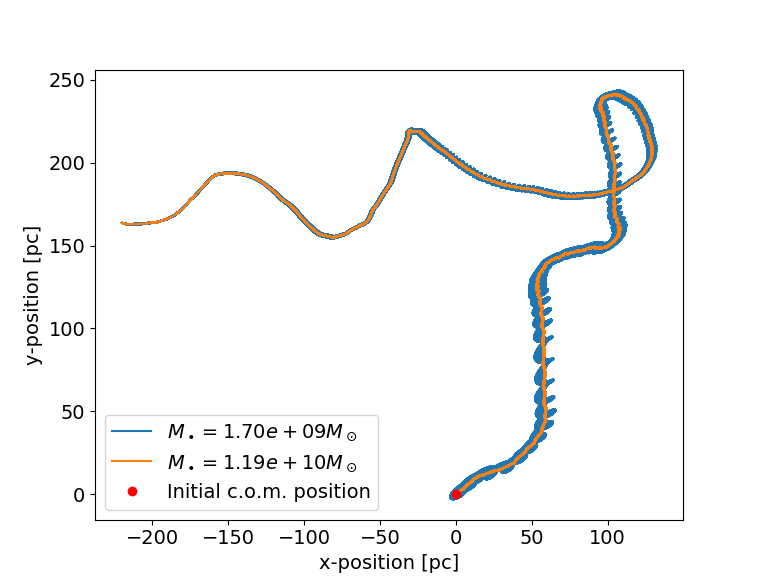
\includegraphics[width=0.7\textwidth]{Run3_Trajectory.png}	
	\caption{The trajectories of the black holes during "run 3" of the simulation. The coordinates are centred on the initial location of the centre-of-mass of the black hole system. The orange and blue lines show the paths taken by the smaller and larger black holes respectively during the simulation. Both paths show clear spiral patterns which become smaller and smaller as the simulation proceeds. The paths end at the location where the black holes merge, i.e. where the distance between them is $\lesssim 100 R_s$ ($R_s$ is the Schwarzschild radius).}
	\label{figure:run3_traj}
\end{figure}

\begin{figure}[h]
	\centering
	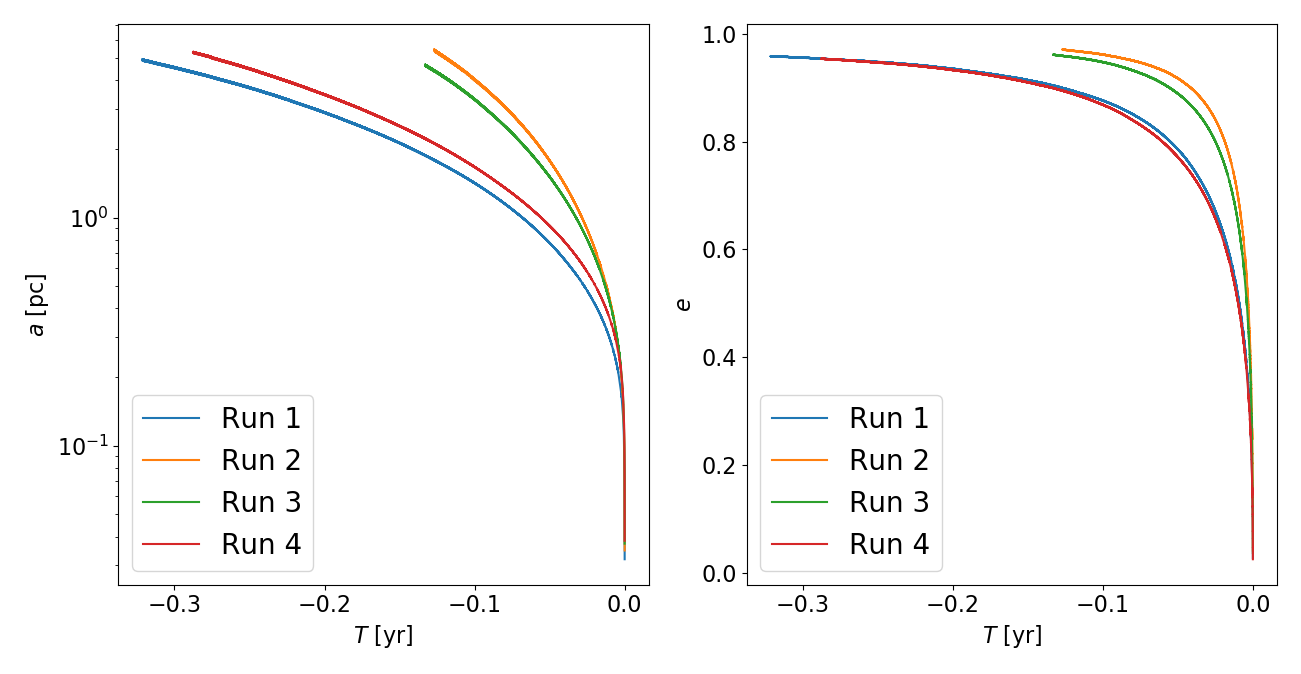
\includegraphics[width=\textwidth]{semi_major_and_ecc.png}
	\caption{The semi-major axes (left) and eccentricities (right) of the black hole systems in simulation runs 1-4 as a function of time. The zero position on the x-axis corresponds to the point of time in the simulation, where the black hole merging event happens.}
	\label{figure:semi_and_ecc}
\end{figure}

%Figure \ref{figure:semi_and_ecc} shows the time evolution of the semi-major axis $a$ and the eccentricity $e$ of the binary from every run. The behaviour of both $a$ and $e$ indicate that the binary does actually merge, as the orbits go from highly eccentric to almost circular, and as $a$ declines exponentially.

The most likely obstacle for the complete merging of the black hole is the so-called final-parsec problem; where the hardening of the binary stops when the separation between the two black hoes is $\sim 1 \mathrm{pc}$ during the three-body scattering phase, due to the lack of stellar material that can be ejected. This is assumed to happen, since not only is the binary constantly ejecting the finite amount of stars inside the loss cone (defined in section 2), but the loss cone itself is becoming smaller due to the contracting orbit of the binary.

Figure \ref{figure:semi_and_ecc} shows the time evolution of both the semi-major axis and the eccentricity of the binary orbits from all of the simulation runs. Interestingly enough the semi-major axes of the binaries go far below single parsec scales, meaning that the final-parsec problem doesn't seem to play a part in the evolution of the simulated binaries. This implies the existence of some loss cone refill mechanism that allows  the binary eject more stellar material than what exists in the loss cone to begin with.


\section{Core Size Measurements}

In order to check if a merger remnant is cored or not, we first have to calculate their surface brightness profiles, and then see if they contain surface brightness deficiencies near the centre of the merger. As the "Runs" don't contain stellar data, we use the "Snapshots" for the core analysis. 

We calculate the surface brightness profiles from the snapshots by: changing the coordinate system to centre-of-mass coordinates, projecting the stellar particles onto a plane, and calculating masses inside logarithmically space radial bins to get a radial mass surface density profile. We then do the aforementioned calculations 100 times from random viewing angles and calculate the azimuthal average of the profiles. This allows us to form a smooth mass surface density profile, which we then turn into a surface brightness profile by assuming a mass-to-light ratio of $M/L = 4$ \citep{Rantala2018}.

In figure \ref{figure:surface_brightness}, one can see example surface brightness profiles for all of the snapshots. Looking at the different curves, it seems like the presence of central SMBHs in the merger progenitors does cause some kind of brightness deficiency near the galactic centre of the remnant's surface brightness profile. Not only that, the higher the mass of the central black holes, the larger the surface brightness deficiency seems to be.

\begin{figure}[h]
	\centering
	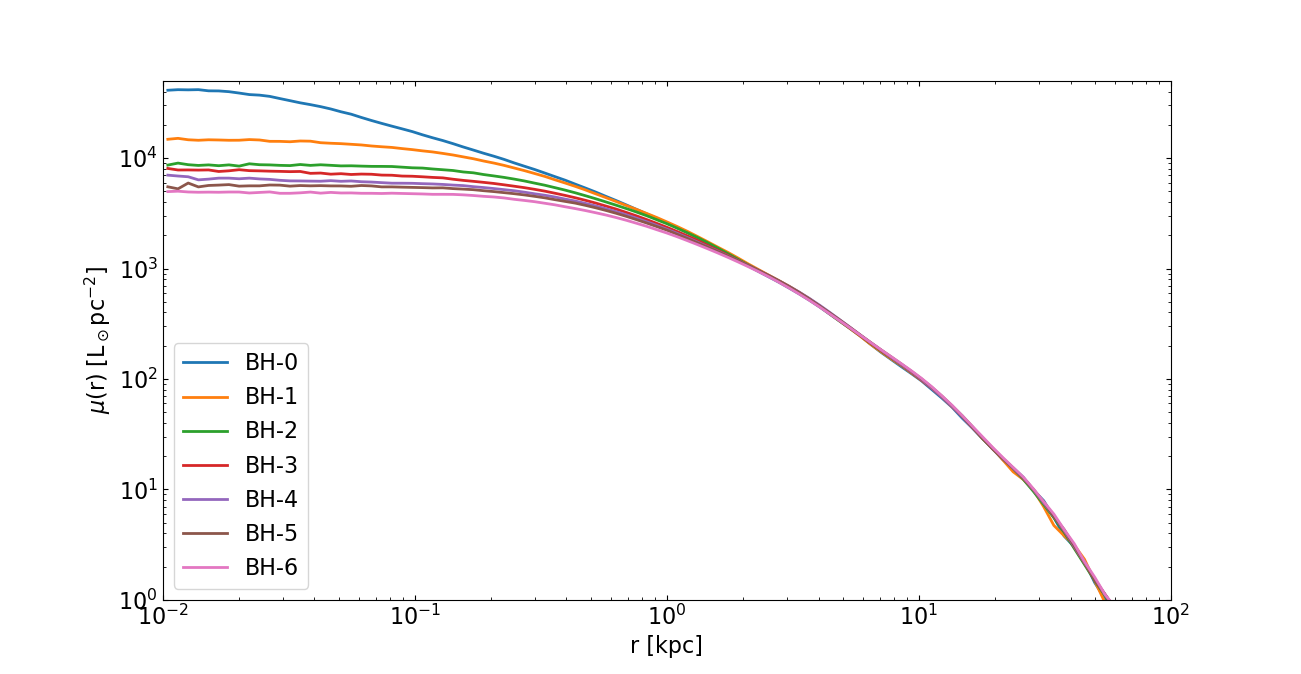
\includegraphics[width=\textwidth]{SurfaceBrightnessProfiles.png}
	\caption{Surface brightness profiles of all of the simulated merger remnants. The profiles were calculated by dividing the remnants into 100 radial bins, and averaging the surface brightness inside the bins through 100 random viewing angles. The luminosity of the particles was estimated by assuming a mass-to-light ratio of $M/L = 4$.}
	\label{figure:surface_brightness}
\end{figure}

The deficiencies found in the surface brightness profiles mentioned above imply the presence of cores, however determining the precise size of the core requires us to find the exact location where the deviations from the expected power-law profile start. This can be done by fitting the calculated profile with a model that is a combination of two power laws: a shallow inner power-law, and a steeper outer power-law. The radius at which the power laws shift, i.e. the break radius $r_b$, is equivalent to the radius of the core. 

There are two commonly used options for modelling the surface brightness profiles. The first one is the core-Sérsic profile \citep{Graham2003}, which can be expressed using the following equation:
\begin{equation}
\mu(r) = \mu' \left[ 1 + \left( \frac{r_b}{r} \right)^\alpha \right]^{\gamma / \alpha} \exp \left\lbrace -b_n \left[ \left( r^\alpha + r_b^\alpha \right) / r_e^\alpha \right]^{1/(\alpha n)} \right\rbrace, \label{eq:core-sersic}
\end{equation}
where $r_b$ is the break radius, $\gamma$ is the logarithmic slope of the inner power-law, $\alpha$ controls the sharpness of the transition between the two power-laws, $r_e$ and $n$ are the effective half-mass radius and the Sérsic index of the outer power-law, and the normalization factor $\mu'$ is defined by:
\begin{equation}
\mu' = \mu_b 2^{-\gamma/\alpha} \exp \left[ b_n \left( 2^(1/\alpha) r_b/r_e \right)^{1/n} \right], 
\label{eq:mu_dot}
\end{equation}
where $\mu_b$ is the surface brightness at the break radius. 

The second option is using the so called Nuker profile \citep{Lauer1995}:
\begin{equation}
\mu(r) = 2^{(\beta - \gamma) / \alpha} \mu_b \left( \frac{r_b}{r} \right)^\gamma \left[ 1 + \left( \frac{r}{r_b} \right)^\alpha \right]^{(\gamma - \beta)/\alpha},
\label{eq:nuker}
\end{equation}
where $r_b$ is once again the break radius, $\mu_b$ is the surface brightness at the break radius, $\beta$ and $\gamma$ are the logarithmic slopes of the power-laws inside and outside of the break radius respectively, and $\alpha$ is the sharpness of the transition between the two slopes.

\begin{figure}[h]
	\centering
	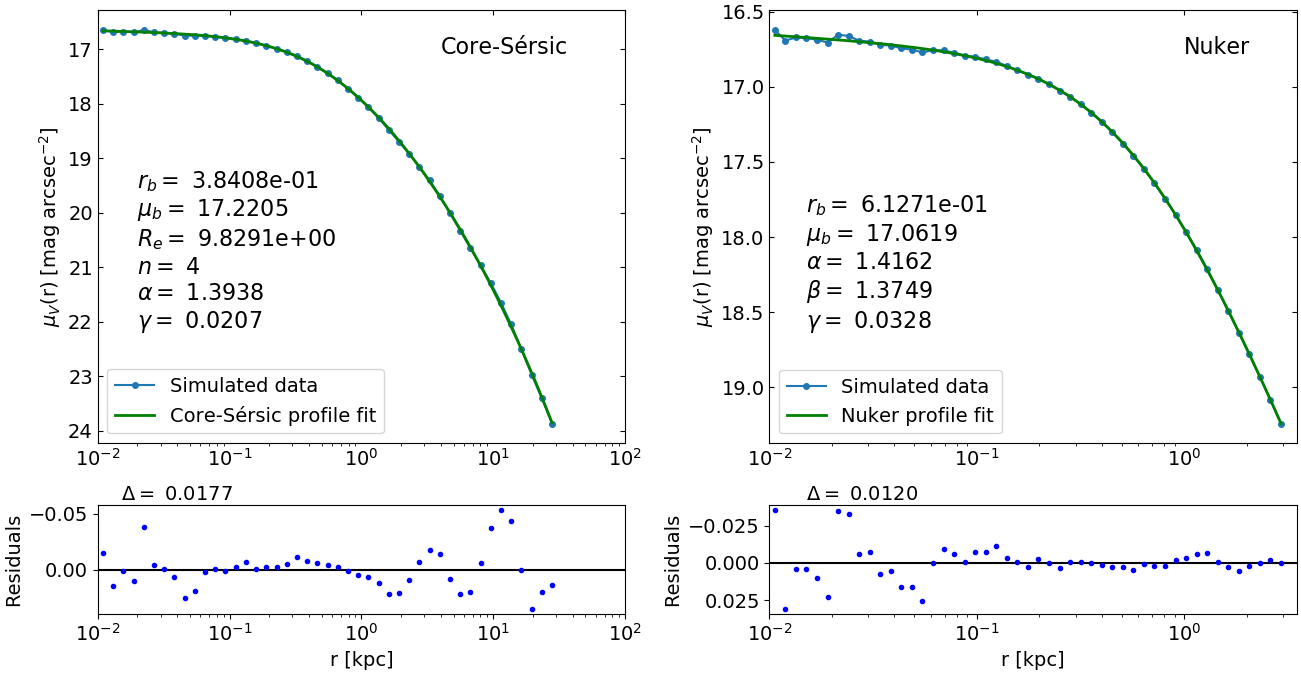
\includegraphics[width=\textwidth]{core_nuker_fits.png}
	\caption{Core-Sérsic and Nuker profile fits of surface brightness profiles calculated from Snapshot 3 (top-left and top-right figures). The best fit parameters are written on the figures, and are in the same units as the axes (i.e. $r_b$ and $R_e$ in kilo-parsecs, and $\mu_b$ in V-band magnitudes per arc-second squared). The relative residuals of the fits are plotted under their respective figures. The delta describes the root-mean-square of the residuals.}
	\label{figure:core_nuker}
\end{figure}

We calculate the core radii of the merger remnants by using the "Levenberg-Marquardt" fitting algorithm to fit both the core-Sérsic model and the Nuker model to the remnant's surface brightness profile. Figure \ref{figure:core_nuker} shows a comparison of the resulting fits for snapshot 3 (refer to table \ref{table:runs_and_snaps}), while figures \ref{figure:all_core} and \ref{figure:all_nuker}, located in the appendix, show the fits for every snapshot that contains SMBH binaries. The values of the best-fit parameters are written on the figures, and looking at them, it is clear that the exact value of the best-fit break radius, i.e. the core radius estimate, depends quite heavily on the used model.

Which model is better for estimating the size of the core is up for debate \citep{Lauer2007, Dullo2012}. While the RMS of the relative residuals seems to be consistently (although just marginally) smaller for the Nuker model when compared to the RMS for the core-Sérsic model (compare figures \ref{figure:all_core} and \ref{figure:all_nuker}), one also has to take into account that in the Nuker model the best-fit value for $r_b$ is highly dependent on the fitting range \citep{Graham2003Nuker}. Furthermore, as stated by \cite{Rantala2018}, in order to get sensible values for all of the model parameters, the fitting range of the Nuker model has to be narrowed down closer to the galactic core ($\alpha \lesssim 1$ might prevent the model from describing the profile as a combination of two power-laws).

One could also estimate the size of the core without model fitting by using the so-called "cusp radius" $r_\gamma$, which is the radius at which the negative logarithmic slope of the surface brightness profile $\gamma'$ equals $1/2$ \citep{Carollo1997, Lauer2007Cusp}. The cusp radius $r_\gamma$ is also an estimation for the location where the inner power-law of the profile changes into the outer power-law, and thus equates to the core radius. 

We calculate $r_\gamma$ for all of the snapshots with SMBH binaries by calculating the first derivative (gradient) of the surface brightness profiles, and then using a "Nelder-Mead" minimization algorithm to find the radius, at which the gradient gets the value $-1/2$. 

Figure \ref{figure:radii_comparison} compares the core radius estimates from each of the three methods for every merger remnant from the snapshots. The break radii from the Nuker fits are consistently larger than the other core radius estimates, while also being the ones that, in general, agree least with the other values. Nevertheless, a clear trend of the size of the core growing with the merger progenitors' central SMBH masses can be seen.

\begin{figure}[h]
	\centering
	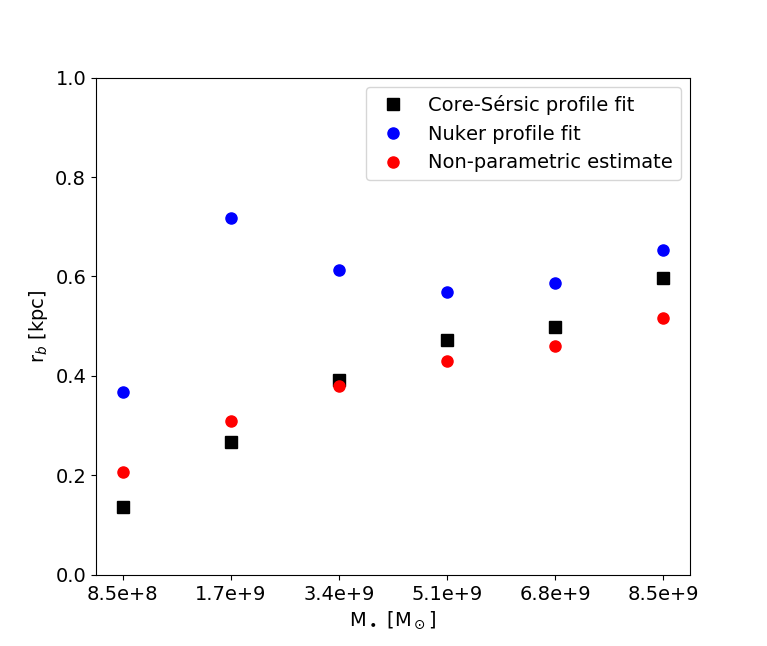
\includegraphics[width=0.7\textwidth]{rb_mass_relation.png}
	\caption{Comparison of core radii of the merger remnants, gained through three different methods: Core-Sérsic profile fitting (black squares), Nuker profile fitting (blue circles) and  finding the "cusp radius" (red circles). The x-axis shows the masses of the central SMBHs of the merger progenitors.}
	\label{figure:radii_comparison}
\end{figure}

\section{Velocity Anisotropy}

%\begin{figure}[h]
%	\centering
%	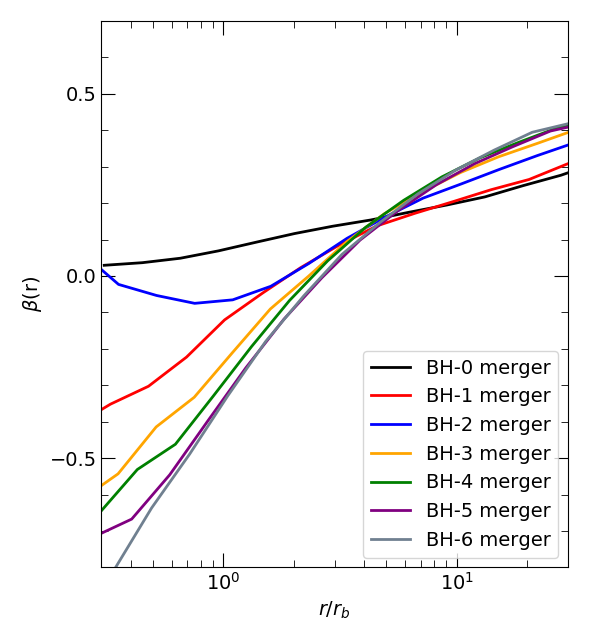
\includegraphics[width=0.9\textwidth]{beta.png}
%	\caption{Velocity anisotropy (beta) profiles of the simulated merger remnants with central black holes.}
%\end{figure}

One way of adding to the evidence that a galaxy has formed a core through core scouring by binary black holes, is to study its velocity anisotropy profile defined in \cite{BinneyTremaine}:
\begin{equation}
\beta(r) = 1 - \frac{\sigma_\theta^2 - \sigma_\phi^2}{2\sigma_r^2} = 1 - \frac{\sigma_t^2}{\sigma_r^2}, \label{eq:beta}
\end{equation}
where $\sigma_\theta$, $\sigma_\phi$ and $\sigma_r$ are velocity dispersions in the spherical coordinates, and $\sigma_t = \sqrt{(\sigma_\theta^2 + \sigma_\phi^2) / 2}$ is the tangential velocity dispersion. The $\beta$ parameter describes the relation between objects in radial and tangential orbits around the black hole binary, where a negative $\beta$ shows an abundance of tangential orbits, and positive an abundance of radial orbits. 

Figure \ref{figure:beta_no_rb} shows $\beta$-profiles calculated from all of the merger remnant snapshots using equation \ref{eq:beta}. According to the profiles, the outer areas of the remnants are dominated by radial orbits, while the majority of orbits near the centre are tangential.

\begin{figure}[h]
	\centering
	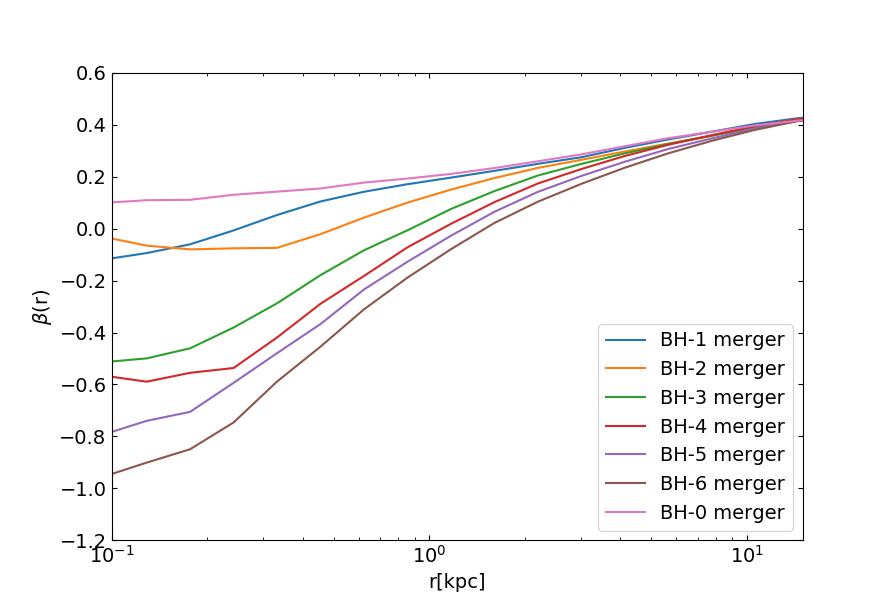
\includegraphics[width=0.9\textwidth]{beta_no_rb.png}
	\caption{Velocity anisotropy (beta) profiles of the simulated merger remnants with central black holes.}
	\label{figure:beta_no_rb}
\end{figure}


As the merging of two galaxies would cause a randomization of the stellar orbits, an area with negative $\beta$ in the merger remnant, would imply that the stars on radial orbits have been ejected from the system. It has been shown that hardening black hole binaries can eject stars on highly radial orbits from the galactic core, which can then in turn cause the outer orbits to become more radial \citep{Quinlan1997, Milosavljevic2001, Thomas2014}.

This could certainly be the reason behind the shapes of the $\beta$ profiles seen in figure \ref{figure:beta_no_rb}. It is clear that the presence of an SMBH binary has an effect on the profiles' shape, as not only is the profile for the merger without a binary the only one completely dominated by radial orbits, but the larger the binary's mass, the steeper the slope of the profile. These properties of the profiles also make sense in the context of ejection of stellar particles by hardening black hole binaries. The larger the masses of the SMBHs in the binary are, the larger the gravitational sphere-of-influence of the binary is, which results in more of the radially orbiting stellar particles being ejected.


\section{Line-of-Sight Kinematics}

In order to make sure that the KETJU simulations produce results equivalent to observations, we analyse the line-of-sight (LOS) kinematics of the "snapshots". We will be analysing four different LOS velocity distribution properties: the average LOS velocity $V_\mathrm{avg}$, the velocity dispersion $\sigma$, and the $h_3$ and $h_4$ parameters which correspond to the skewness and the kurtosis of the distribution respectively. The distribution from which these properties are calculated is defined as the following modified Gaussian function \citep{Rantala2018}:
\begin{equation}
f(v) = I_0 e^{-\gamma^2/2}(1 + h_3 H_3(y) + h_4 H_4(y)), \label{eq:mod_gaussian}
\end{equation} 
where $I_0$ is a normalization constant, $\gamma$ is the central slope of the particle density profile, $y = (v - V_\mathrm{avg})/\sigma$, and $H_3$ and $H_4$ are the third and fourth order Hermite polynomials respectively:
\begin{eqnarray}
H_3(y) = \left(2\sqrt{2}y^3 - 3\sqrt{2}y\right) / \sqrt{6}, \\
H_4(y) = \left(4y^4 - 12y^2 + 3 \right) / \sqrt{24}.
\end{eqnarray}

In order to calculate the above properties, we first define the "line-of-sight" as the intermediate axis of the merger remnants, and orient the remnant accordingly using the inertia tensor. Next, we divide a 2D line-of-sight projection of the remnant into "spaxels" (or simply bins), using the voronoi tessellation algorithm \citep{Cappellari2003}. The shape and size of the spaxels are determined so that each one contains the same signal-to-noise ratio, which in our case is defined as the number of stellar particles. The LOS-velocities inside the spaxels are then made into a histogram, into which we fit the modified Gaussian function described in equation \ref{eq:mod_gaussian}, giving us the values of the LOS-velocity distribution parameters: $V_\mathrm{avg}$, $\sigma$, $h_3$ and $h_4$ for the spaxel in question. Finally, the values of the spaxels can be plotted, giving us 2D voronoi binned maps of all of the four parameters.

Figure \ref{figure:snapshot_0_and_1_IFU} shows the voronoi binned 2D maps of the four LOS velocity distribution parameters for snapshot-0 and snapshot-6, as well as luminosity contours with one magnitude spacing. Similar maps for all of the merger remnant snapshots are in figures \ref{figure:all_voronoi_1} and \ref{figure:all_voronoi_2} in the appendix.

The IFU maps in figures \ref{figure:all_voronoi_1} and \ref{figure:all_voronoi_2} show that the line-of-sight kinematics of the simulated merger remnants are far from isotropic, with some of the maps from simulations with larger central SMBHs showcasing counter-rotating central regions, or "kinematically distinct cores" (KDC). These features, alongside the relatively low average LOS-velocities, are found in galaxies called "slow rotators" \citep{Emsellem2007}. Slow rotator galaxies are early type galaxies which are assumed to have been formed through gas-poor "dry" mergers \citep{Emsellem2007, Cappellari2007}; processes not unlike the ones simulated in our simulations. As such, the merger remnants being slow rotators is a somewhat expected result, however it nonetheless implies that the KETJU simulations do produce physically accurate results.

\begin{figure}
	\centering
	\begin{subfigure}[b]{0.49\textwidth}
		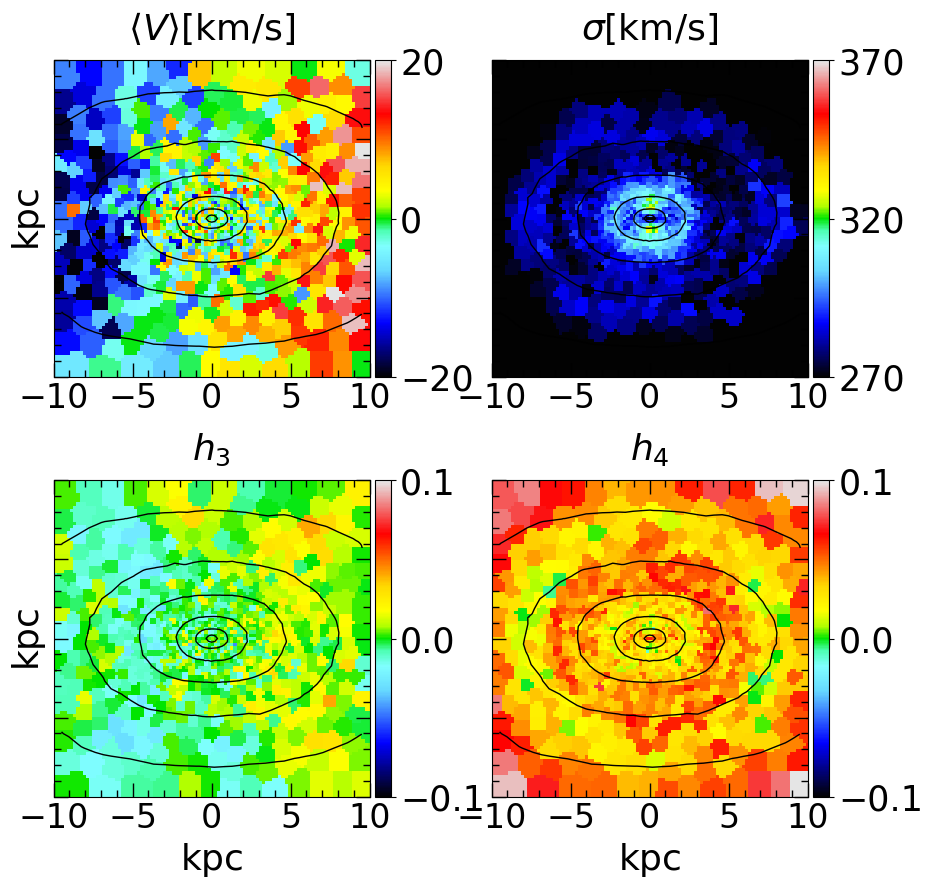
\includegraphics[width=\textwidth]{BH_0.png}
		\caption{Snapshot-0}
	\end{subfigure}
	\begin{subfigure}[b]{0.49\textwidth}
		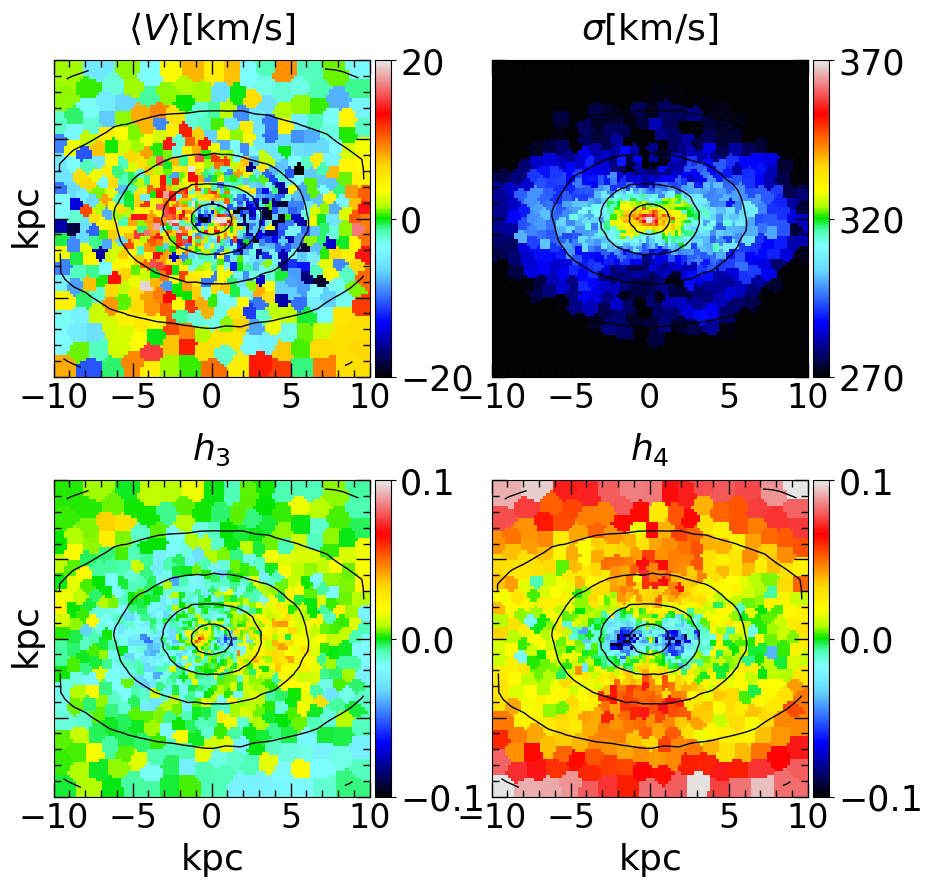
\includegraphics[width=\textwidth]{BH_6.png}
		\caption{Snapshot-6}
	\end{subfigure}
	\caption{IFU-maps of average LOS-velocities, velocity dispersion, $h_3$ parameters and $h_4$ parameters from two simulated merger remnants. The four maps on the left are from a merger simulation where the progenitor galaxies had no central SMBHs, where as the four on the right are from a simulation with progenitor galaxies containing $M_\bullet = 8.5 \times 10^9 M_\odot$ central black holes.}
	\label{figure:snapshot_0_and_1_IFU}
\end{figure}

Further analysis of the nature of the simulated mergers' rotation can be done by looking at the $\lambda_R$ parameter, which describes the angular momentum of a galaxy \citep{Emsellem2007}. More importantly, the parameter allows us to differentiate between the aforementioned slowly rotating galaxies and so-called fast rotators (see figure \ref{figure:obs_IFU}) \citep{Emsellem2007}. The parameter itself is defined in a general form as:
\begin{equation}
\lambda_R \equiv \frac{\langle R |V| \rangle}{\langle R \sqrt{V^2 + \sigma^2} \rangle}, \label{eq:general_lambdar}
\end{equation}
where $R$ is the projected distance from the galactic centre, $V$ is velocity, $\sigma$ is the velocity dispersion, and $\langle \; \rangle$ denote that the nominator and denominator of the equation are velocity weighted means. However, as most of the observational kinematic analysis of galaxies is done through binned 2D spectroscopy, and as the IFU-maps made from our simulations are produced the same way as the ones gained through observations, we will be using the following version of the equation:
\begin{equation}
\lambda_R = \frac{\sum^{N_p}_{i=1} F_i R_i |V_i|}{\sum^{N_p}_{i=1} F_i R_i \sqrt{V_i^2 + \sigma^2_i}}, \label{eq:binned_lambdar}
\end{equation}
where $F_i$, $R_i$, $V_i$ and $\sigma_i$ are the flux, projected distance from the galaxy centre, velocity and velocity dispersion of the $i$th bin, and $N_p$ is the number of bins. In the case of our simulations, the $N_p$ bins used are of course the voronoi bins described earlier in this section. 

\begin{figure}
	\centering
	\begin{subfigure}[b]{0.49\textwidth}
		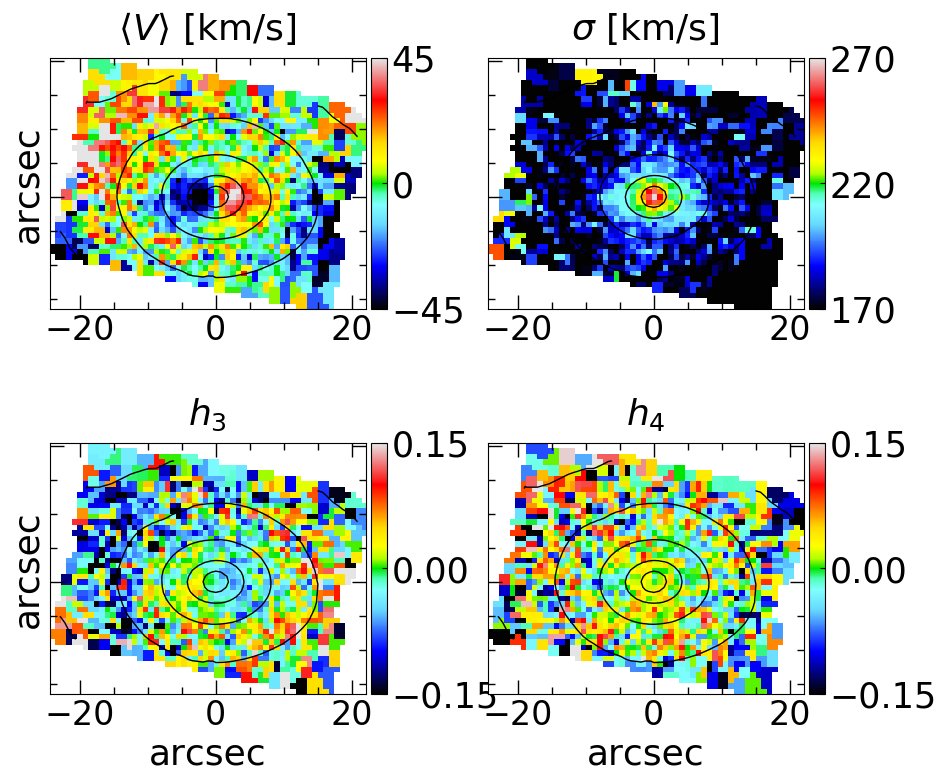
\includegraphics[width=\textwidth]{NGC3414_r6_voronoi.png}
		\caption{NGC 3414}
	\end{subfigure}
	\begin{subfigure}[b]{0.49\textwidth}
		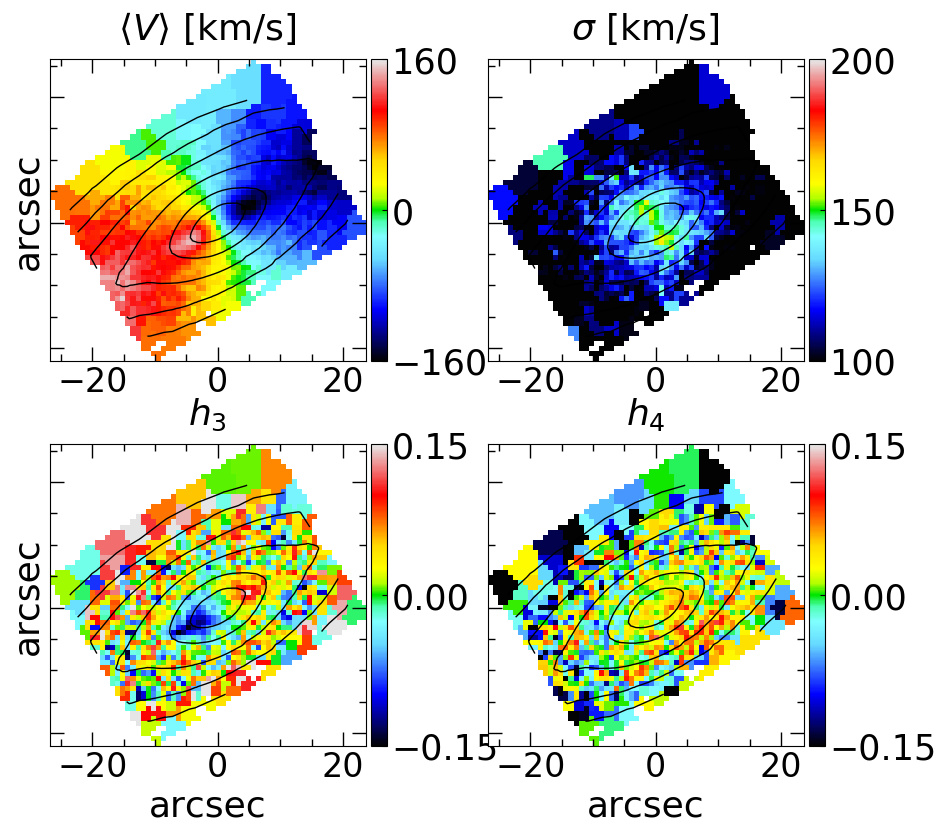
\includegraphics[width=\textwidth]{NGC4111_r1_voronoi.png}
		\caption{NGC 4111}
	\end{subfigure}
	\caption{Comparison between the IFU-maps of known slow (NGC 3414) and fast rotator (NGC 4111) galaxies from the $\mathrm{ATLAS^{3D}}$ survey. The maps show the average LOS-velocities, velocity dispersion, $h_3$ parameters and $h_4$ parameters of NGC 3414 \citep{Emsellem2004} and NGC 4111 \citep{Cappellari2011}.}
	\label{figure:obs_IFU}
\end{figure}

Determining whether a galaxy is either a fast or a slow rotator using $\lambda_R$ is done by comparing the value that the parameter gets at the galaxy's effective radius, to some pre-defined threshold. The original threshold used for differentiating the two rotator types is: $\lambda_{Re} < 0.1$, where $\lambda_{Re}$ is $\lambda_R$ at the effective radius, and where galaxies fulfilling the condition are classified as slow rotators \citep{Emsellem2007}. Later revisions by \cite{Emsellem2011} and \cite{Cappellari2016} take the ellipticity ($\epsilon$) of the galaxy into account, and define the threshold as being either $\lambda_{Re} < 0.31\sqrt{\epsilon}$ or $\lambda_{Re} < 0.08 + \epsilon/4$ for $\epsilon < 0.4$ respectively. Through including the ellipticity in the threshold, the revisions account for increased anisotropy in the kinematics of flatter galaxies. The latter threshold then improves on the former by reducing the risk of misidentifying round non regular slow rotators as fast rotators.

Since two of the three aforementioned slow rotator thresholds require us to know the ellipticity of the galaxy, we calculate the simulated merger remnants' ellipticities before analysing their rotation. The ellipticity calculations are done using a method described in \cite{Zemp2011}, which uses the shape tensor:
\begin{equation}
\mathbf{S} = \frac{\int_V \rho(\mathbf{r}) \omega(\mathbf{r}) \mathbf{r} \mathbf{r}^T \; dV }{\int_V \rho{\mathbf{r}} \; dV},
\end{equation}
where $\mathbf{r}$ is position from the galactic centre, $\rho(\mathbf{r})$ is the mass density, $V$ is the volume of an enclosed ellipsoid with the elliptical radius $r_\mathrm{ell}$, and where the weighting function $\omega(\mathbf{r}) = 1$. The eigenvalues of the shape tensor correspond to $a^2/3$, $b^2/3$ and $c^2/3$; where $a$, $b$ and $c$ are the semi-principal axes; and which can be used to calculate the ellipticity as $\epsilon = 1 - b/a$. 

However, simply calculating the shape tensor and getting the eigenvalues isn't possible, as the elliptical radius is defined, in part, using the axis ratios $a/b$ and $a/c$:
\begin{equation}
r_\mathrm{ell} = \sqrt{x_\mathrm{ell}^2 + \frac{y_\mathrm{ell}^2}{(b/a)^2} + \frac{z_\mathrm{ell}^2}{(c/a)^2}}.
\end{equation}
This means that we have to turn the calculation into an iterative process by starting with $b/a = c/a = 1$ for the initial value of $r_\mathrm{ell}$, and calculating new shape tensor eigenvalues using previously gained axis ratios until the values of the ratios start to converge. 

We calculate $\lambda_{Re}$ and $\epsilon_e$, i.e. the ellipticity at the effective radius (the ellipticity is calculated using $r_\mathrm{ell} = R_e$, and a convergence criterion of a difference smaller $10^-3$ between consequent axis ratios), for every merger simulation snapshot and plot them against each other, alongside the previously mentioned slow rotator thresholds, and observations from the $\mathrm{ATLAS^{3D}}$-survey \citep{Cappellari2011}. The resulting plot can be seen in figure \ref{figure:lambda_epsilon}. 

\begin{figure}[h]
	\centering
	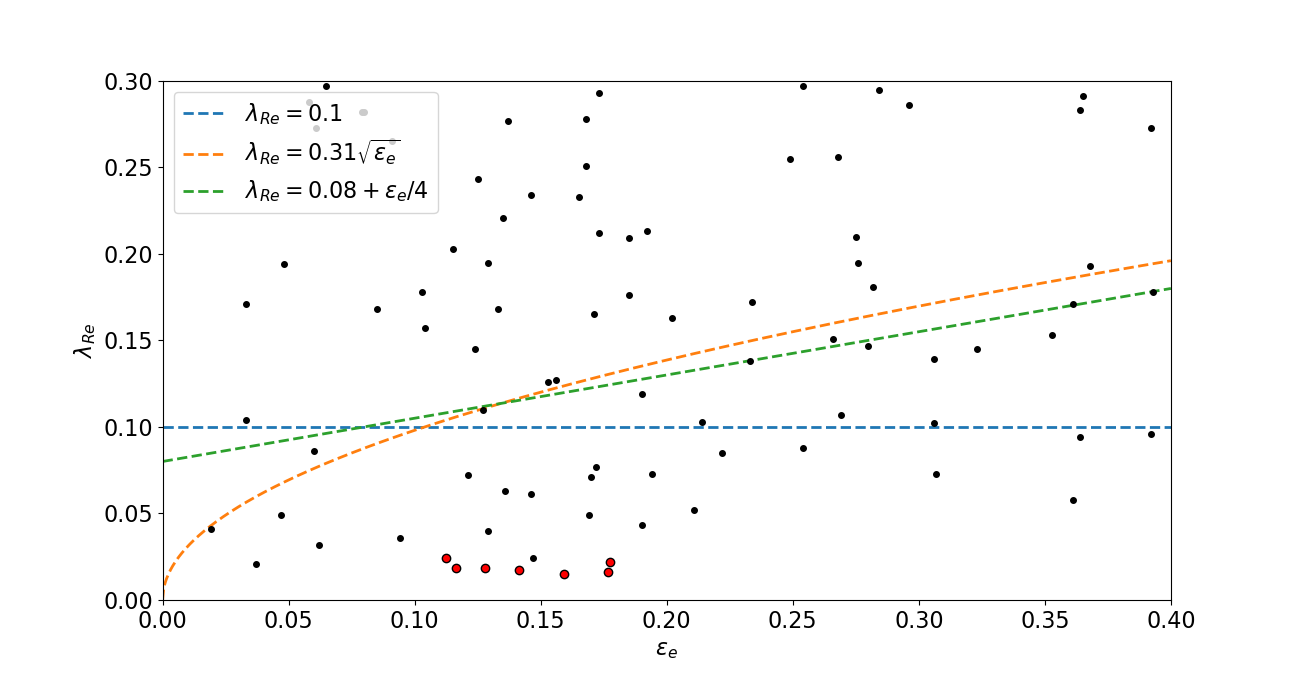
\includegraphics[width=\textwidth]{lambda_epsilon.png}
	\caption{The values of the $\lambda_{\mathrm{Re}}$-parameter of galaxies, plotted against their ellipticity at the effective radius. The red dots correspond to the simulated merger remnants, where as the black dots correspond to galaxies observed in the $\mathrm{ATLAS^{3D}}$-survey \citep{Cappellari2011, Emsellem2011}. The dashed lines display different slow rotator thresholds as a function of ellipticity \citep{Emsellem2007, Emsellem2011, Cappellari2016}.}
	\label{figure:lambda_epsilon}
\end{figure}

Regardless of the threshold used for differentiating between slow and fast rotators, figure \ref{figure:lambda_epsilon} shows us that all of the simulated merger remnants are clearly classified as slow rotators. This agrees well with the kinematic anisotropies seen in the IFU maps, which also implied a slow rotator classification for the remnants.

\section{Comparison to NGC 1600}

As the physical properties of the merger progenitors are modelled after NGC 1600, it is interesting to see how the results from the simulations compare to actual observations of NGC 1600. We are mainly comparing the observations to the simulated merger remnant from "Snapshot-6", as the mass of the SMBH binary in the simulation in question is equivalent to the assumed mass of the central SMBH in NGC 1600 ($M_\bullet = 1.7 \times 10^7 M_\odot$) \citep{Thomas2016}.

\begin{figure}[h]
	\centering
	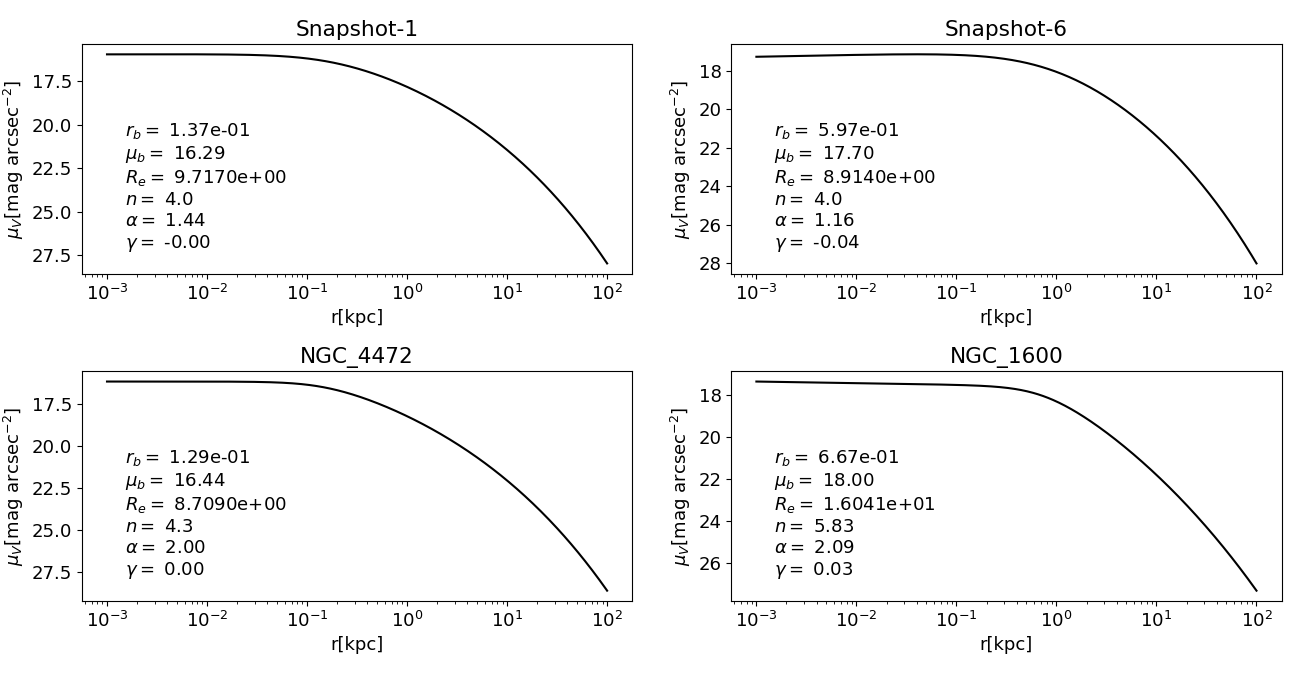
\includegraphics[width=\textwidth]{core_sersic_fits_obs_and_sim.png}
	\caption{Core-Sérsic profile fits of surface brightness profiles calculated from either merger simulation results (top figures) or observed galaxies (bottom figures). The respective fit parameters are written on the figures in units that correspond to the axes. The progenitors of the top-left simulation contained $8.5 \times 10^8 M_\odot$ mass central SMBHs, and $8.5 \times 10^9 M_\odot$ mass central SMBHs in the top-right simulation. The parameters for NGC 1600's profile (bottom right), are changed from the units used by \cite{Thomas2016} to the above by assuming $V - R = 0.5$ (the same assumption being done by \cite{Lauer2007}), and by using the distance $D = 64 \mathrm{Mpc}$ \citep{Thomas2016} in order to define the relation between arc seconds and parsecs. As one can see, the profiles gained from simulations and observations are quite similar to each other.}
	\label{figure:coresersic_sim_obs}
\end{figure}

Figure \ref{figure:coresersic_sim_obs} shows the core-Sérsic profile fits of the surface brightness profiles alongside the best-fit parameters from Snapshot-6 and NGC 1600 as well as from Snapshot-1 and NGC 4472. Comparing the profiles of Snapshot-6 and NGC 1600, one can see unmistakeable similarities. Not only are the shapes of the profiles extremely similar, apart from the larger core and effective radii the best-fit parameters are also quite closely related.

A further comparison between the physical properties of Snapshot-6 and NGC 1600 can be seen in table \ref{table:snap6_vs_NGC1600}. Once again, apart from the effective radius the physical parameters are extremely similar, as between the simulation and the observations the physical parameters are of the same order of magnitude.

\begin{table}
	\begin{center}
		\scriptsize
		\begin{tabular}{c c c c c c c c c c}
		\hline
		\hline
		Galaxy & $M_\star$ & $M_\bullet$ & $R_e$ & $\mu_e$ & $n$ & 
		$V_\mathrm{LOS}$ & $\sigma_e$ & $\lambda_e$ &
		$\epsilon_e$ \\
		& $[\times 10^{11} M_\odot]$ & $[\times 10^{10} M_\odot]$ &
		[kpc] & [$\mathrm{mag/arcsec^2}$] & & [km/s] & [km/s] & & \\
		(1) & (2) & (3) & (4) & (5) & (6) & (7) & (8) & (9) & (10) \\
		\hline
		Snapshot-6 & $4.960$ & $2 \times 0.85$ & $5.507$ & $20.26$ & $4$ & $6.9$ & $311$ & $0.024$ & $0.11$ \\
		NGC 1600 & $5.0$ & $1.7$ & $\sim 16$ & $\sim 22.8$ & $5.83$ & $3.4$ & 
		$293$ & $0.026$ & $032$ \\
		\hline
		\end{tabular}
	\end{center}
	\caption{Comparison between the physical properties of the simulated merger remnant "Snapshot-6" and the galaxy NGC 1600. The properties described in the columns of the table are explained below, with the sources for the properties of NGC 1600 being written inside the brackets. \\
	(1) Name of the galaxy. \\
	(2) Total stellar mass \citep{Thomas2016}. \\
	(3) Central black hole mass \citep{Thomas2016}. \\
	(4) Effective radius \citep{Thomas2016}. For NGC 1600, the effective radius is changed from arc seconds to kpc by assuming that it is located at the distance of $D = 64 \; \mathrm{Mpc}$ \citep{Thomas2016}. \\
	(5) Surface brightness at the effective radius. Calculated from the best fit core-Sérsic profile parameters given in \cite{Thomas2016}. \\
	(6) Sérsic index from the best fitting core-Sérsic profile fit \citep{Thomas2016}. \\
	(7) Mean line-of-sight velocity inside the effective radius \citep{Bender1994}. \\
	(8) Velocity dispersion inside the effective radius \citep{Veale2017veldisp}. For "Snapshot-6", the given velocity dispersion is calculated from a Voronoi binned image as the mean of the velocity dispersion values of the bins located inside the effective radius. \\
	(9) Spin parameter at the effective radius \citep{Veale2018lambda}. \\
	(10) For "Snapshot-6": ellipticity of the galaxy at the effective radius; and for GC 1600: luminosity weighted ellipticity \citep{Goullaud2018}.
	}
	\label{table:snap6_vs_NGC1600}
\end{table}

Of course, due to the nature in which the merger progenitors were modelled, the physical parameters being similar between the simulated merger remnant and NGC 1600 is the expected result. The only real surprise is that the core size of NGC 1600 is almost three times larger than the one from Snapshot-6.


\section{Implications}


\chapter{Conclusions}

\appendix

\chapter{Figures}

\begin{figure}
	\centering
	\begin{subfigure}[b]{0.49\textwidth}
		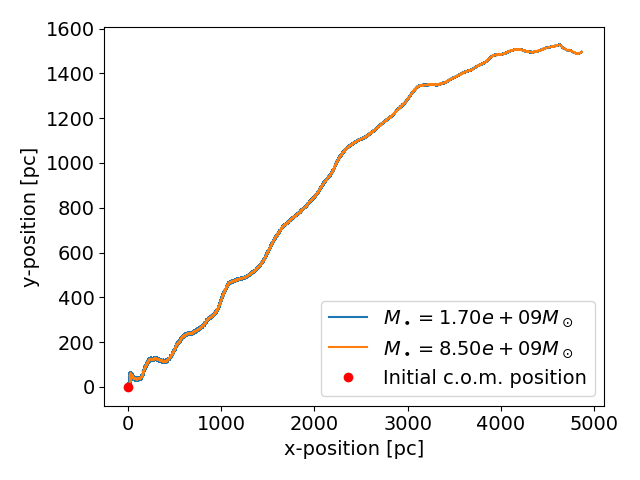
\includegraphics[width=\textwidth]{Run1_Trajectory_small.png}
		\caption{Run 1}
	\end{subfigure}
	\begin{subfigure}[b]{0.49\textwidth}
		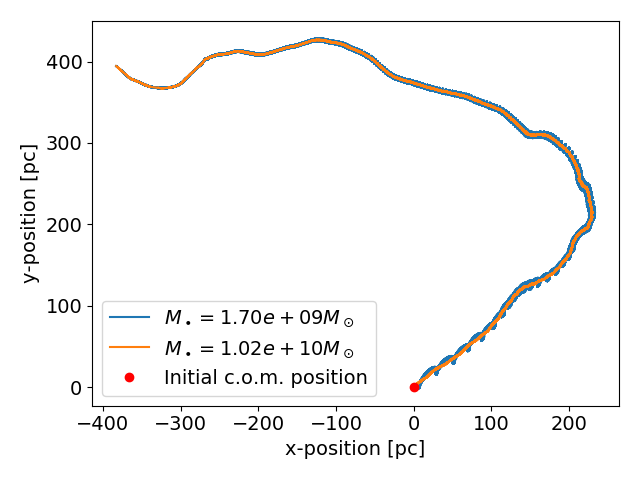
\includegraphics[width=\textwidth]{Run2_Trajectory_small.png}
		\caption{Run 2}
	\end{subfigure}
	\begin{subfigure}[b]{0.49\textwidth}
		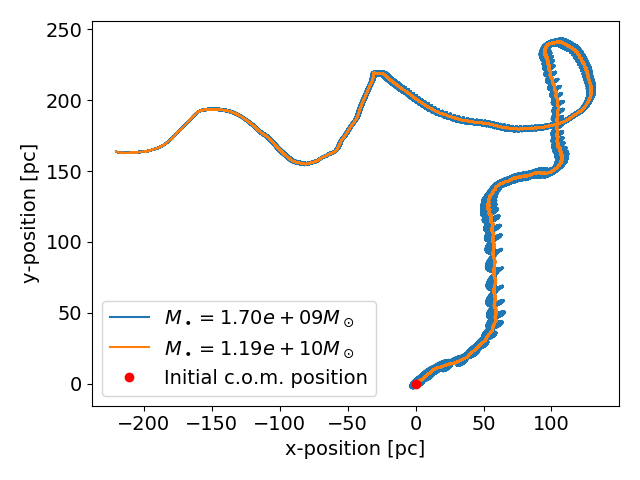
\includegraphics[width=\textwidth]{Run3_Trajectory_small.png}
		\caption{Run 3}
	\end{subfigure}
	\begin{subfigure}[b]{0.49\textwidth}
		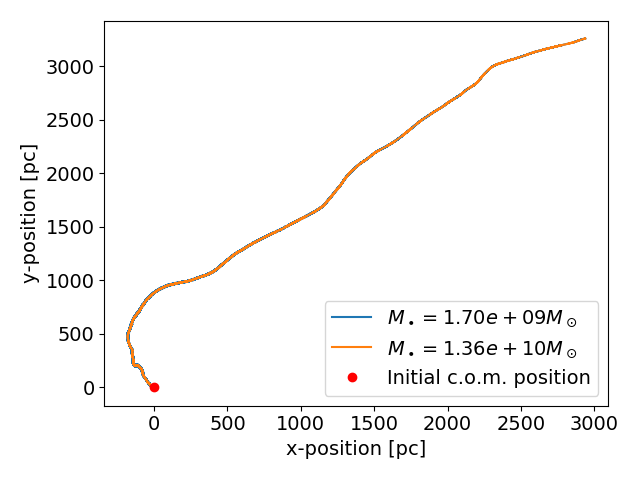
\includegraphics[width=\textwidth]{Run4_Trajectory_small.png}
		\caption{Run 4}
	\end{subfigure}
	\caption{The trajectories of the black holes from simulation runs by \cite{Mannerkoski2019}. The coordinates are centred on the initial location of the centre-of-mass of the black hole system. The orange and blue lines show the paths taken by the smaller and larger black holes respectively during the simulation.}
	\label{figure:all_traj}
\end{figure}

\begin{figure}[h]
	\centering
	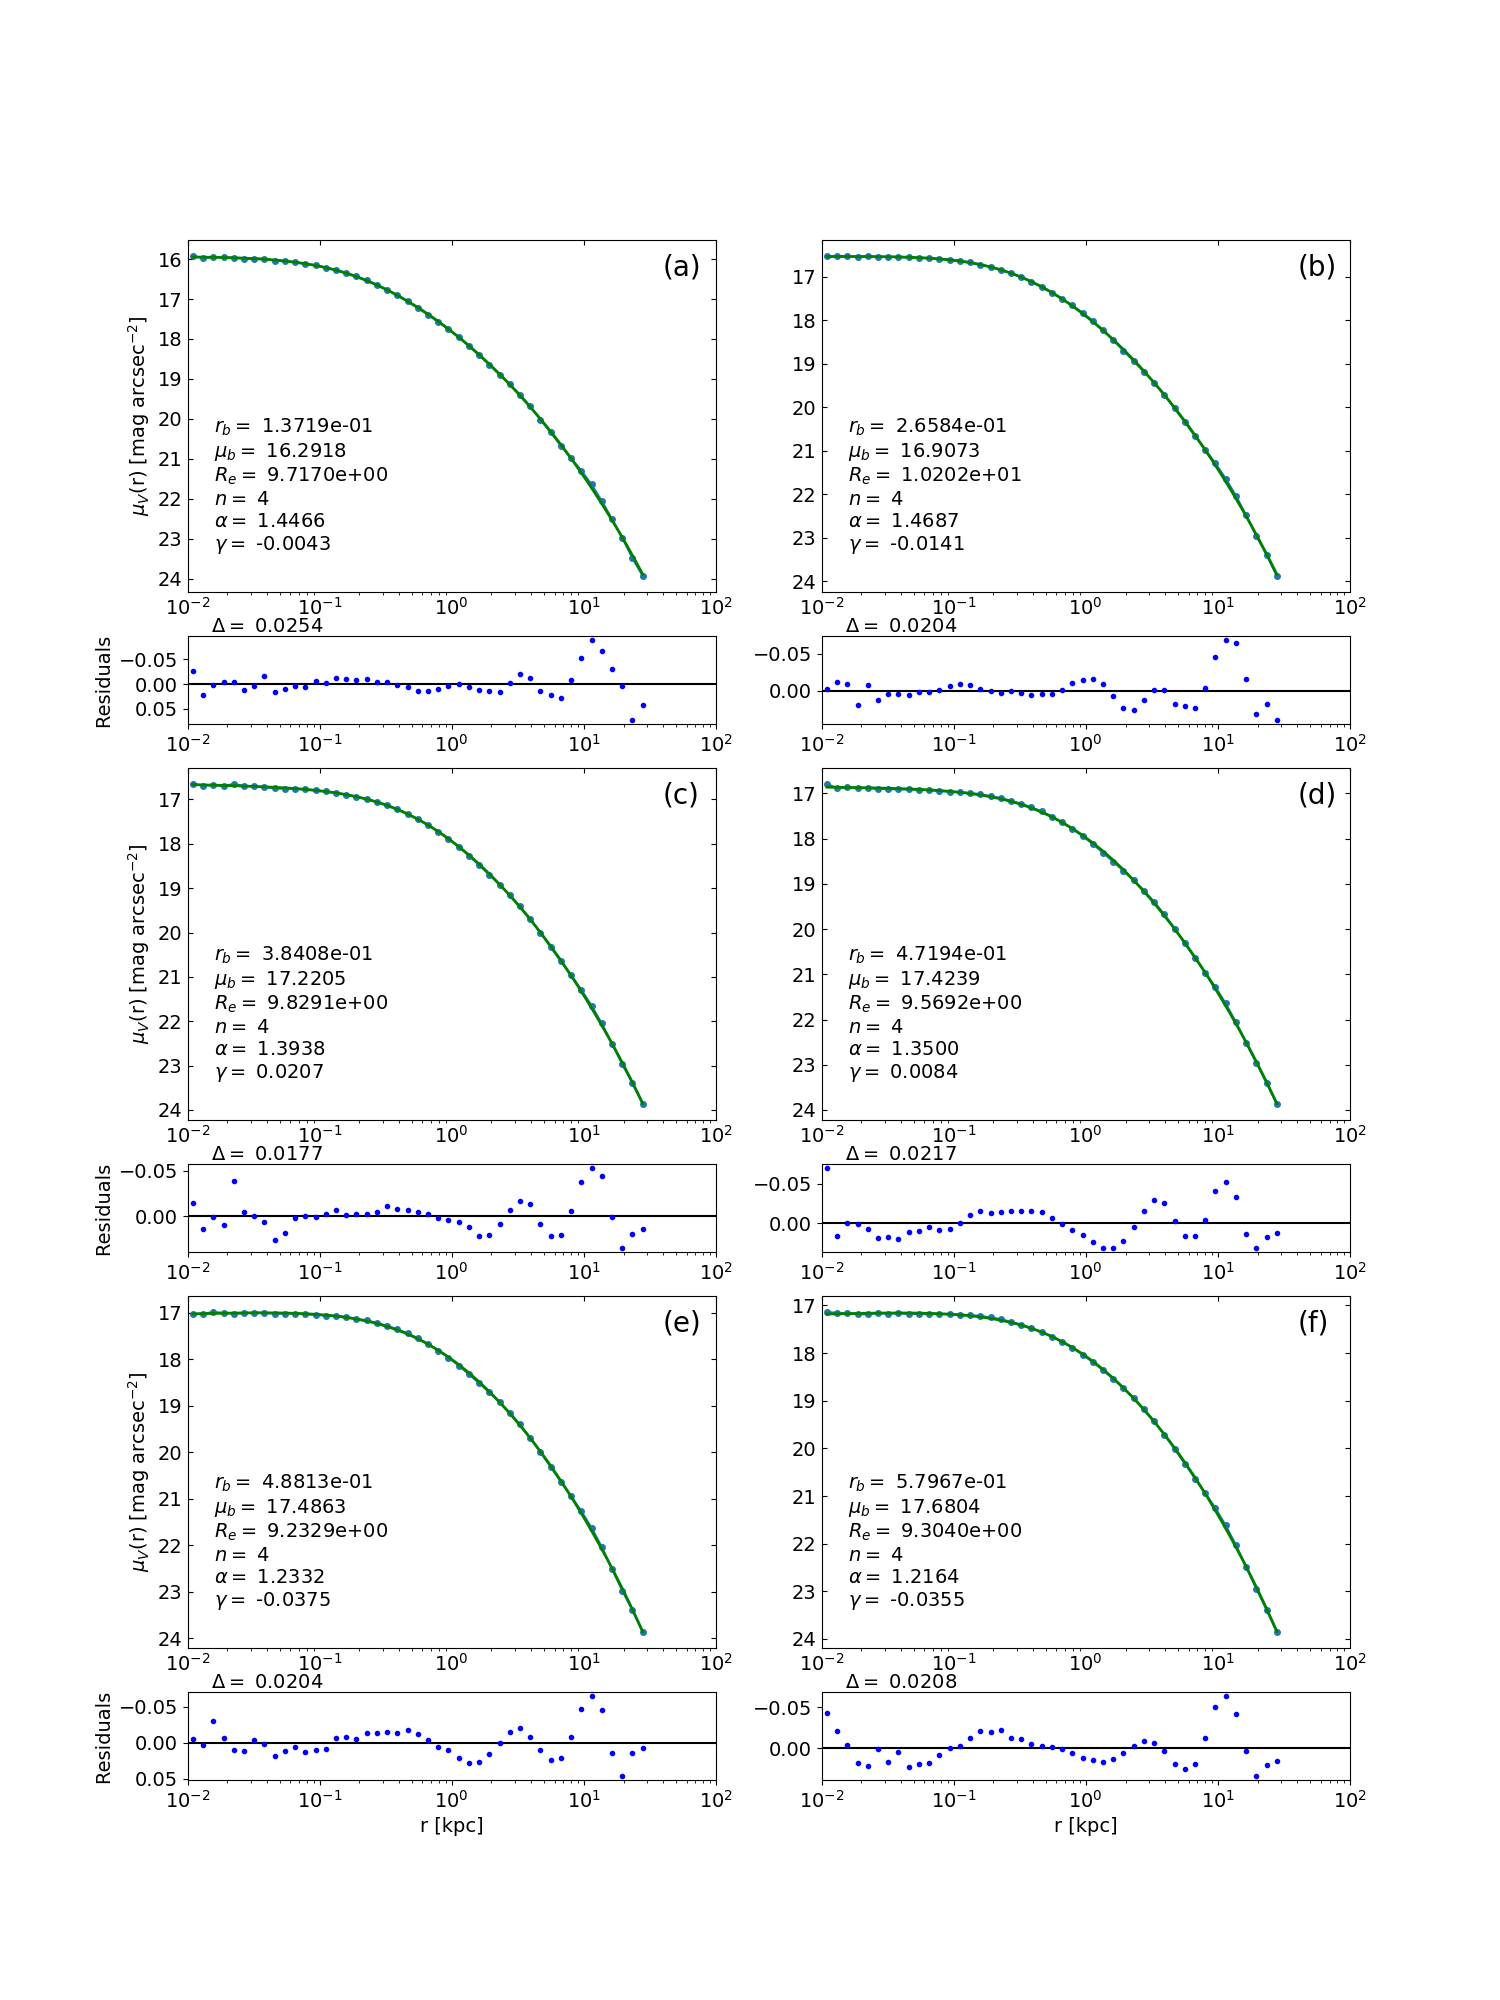
\includegraphics[width=\textwidth]{all_core_profiles.png}
	\caption{Core-Sérsic profile fits of the surface brightness data calculated from all of the individual simulated merger remnants with progenitors containing central supermassive black holes. The letters (a)-(f) denote the different snapshots ((a): Snapshot-1, (b): Snapshot-2, (c): Snapshot-3, (d): Snapshot-4, (e): Snapshot-5, (f): Snapshot-6).}
	\label{figure:all_core}
\end{figure}

\begin{figure}[h]
	\centering
	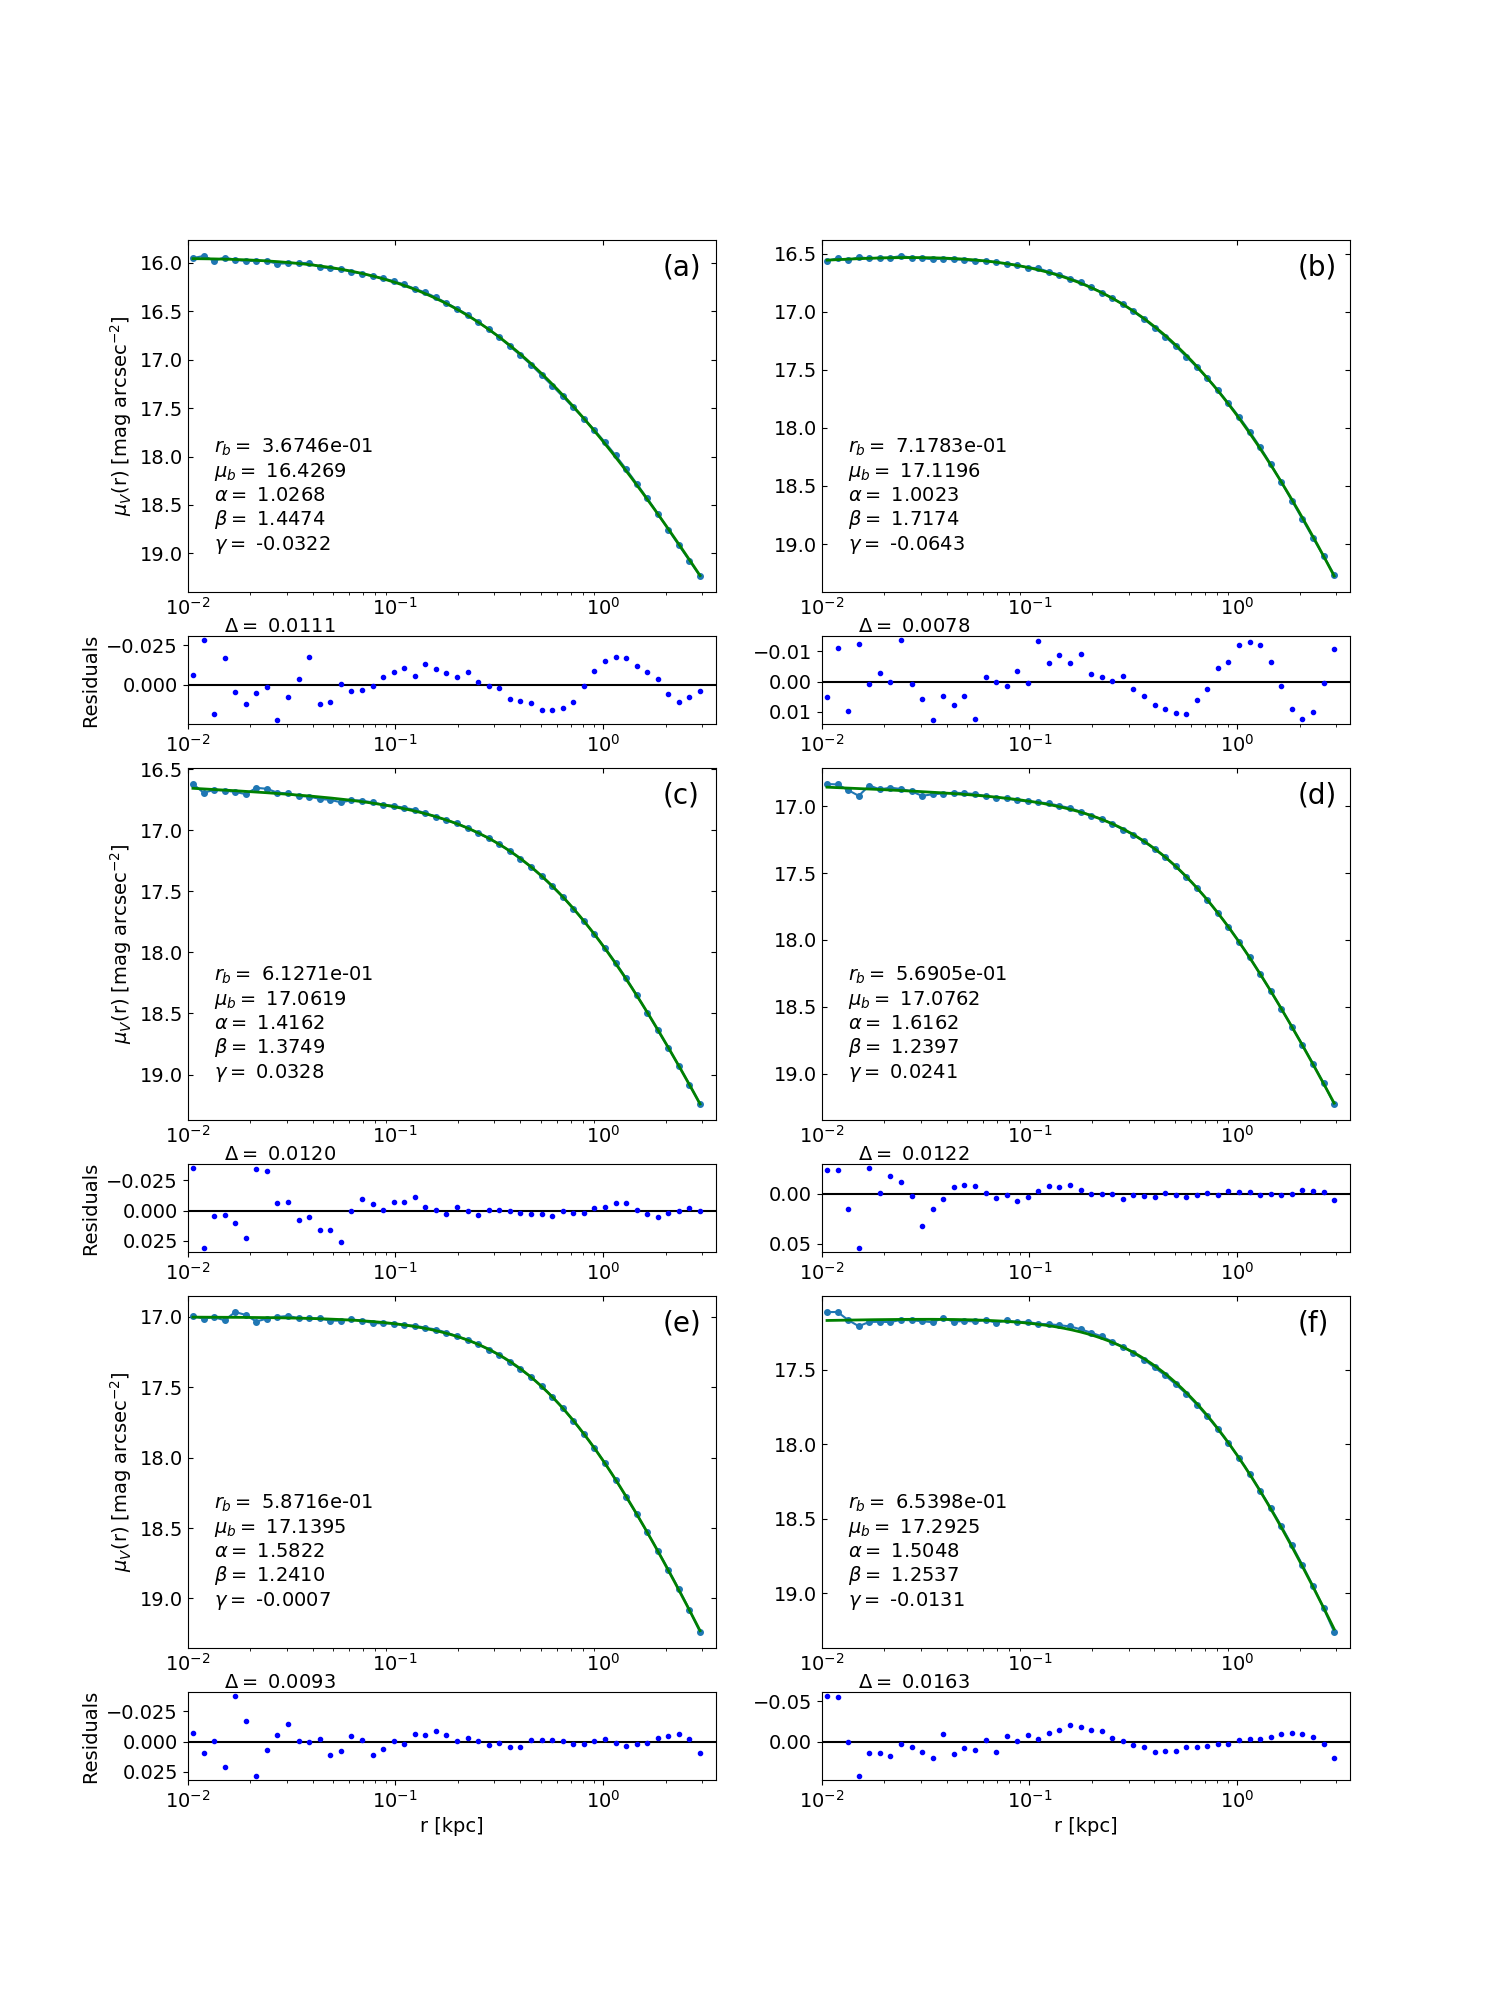
\includegraphics[width=\textwidth]{all_nuker_profiles.png}
	\caption{Nuker profile fits of the surface brightness data calculated from all of the individual simulated merger remnants with progenitors containing central supermassive black holes. The letters (a)-(f) denote the different merger remnants ((a): Snapshot-1, (b): Snapshot-2, (c): Snapshot-3, (d): Snapshot-4, (e): Snapshot-5, (f): Snapshot-6).}
	\label{figure:all_nuker}
\end{figure}

\begin{figure}
	\centering
	\begin{subfigure}[b]{0.49\textwidth}
		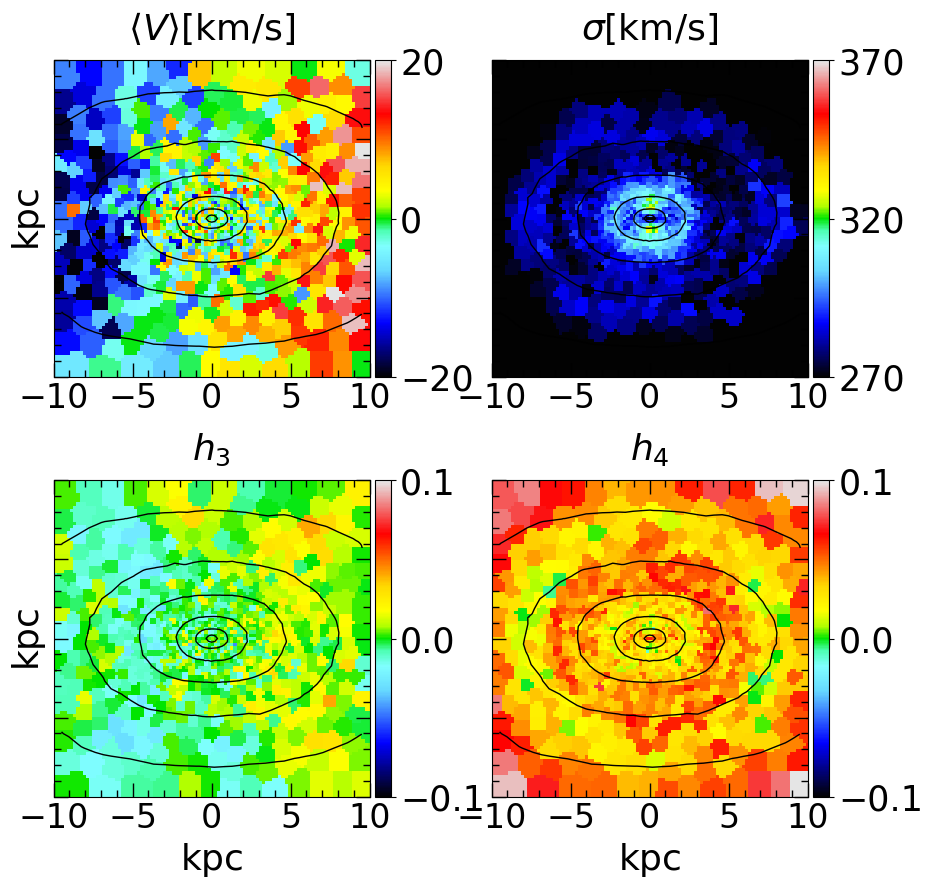
\includegraphics[width=\textwidth]{BH_0.png}
		\caption{Snapshot-0}
	\end{subfigure}
	\begin{subfigure}[b]{0.49\textwidth}
		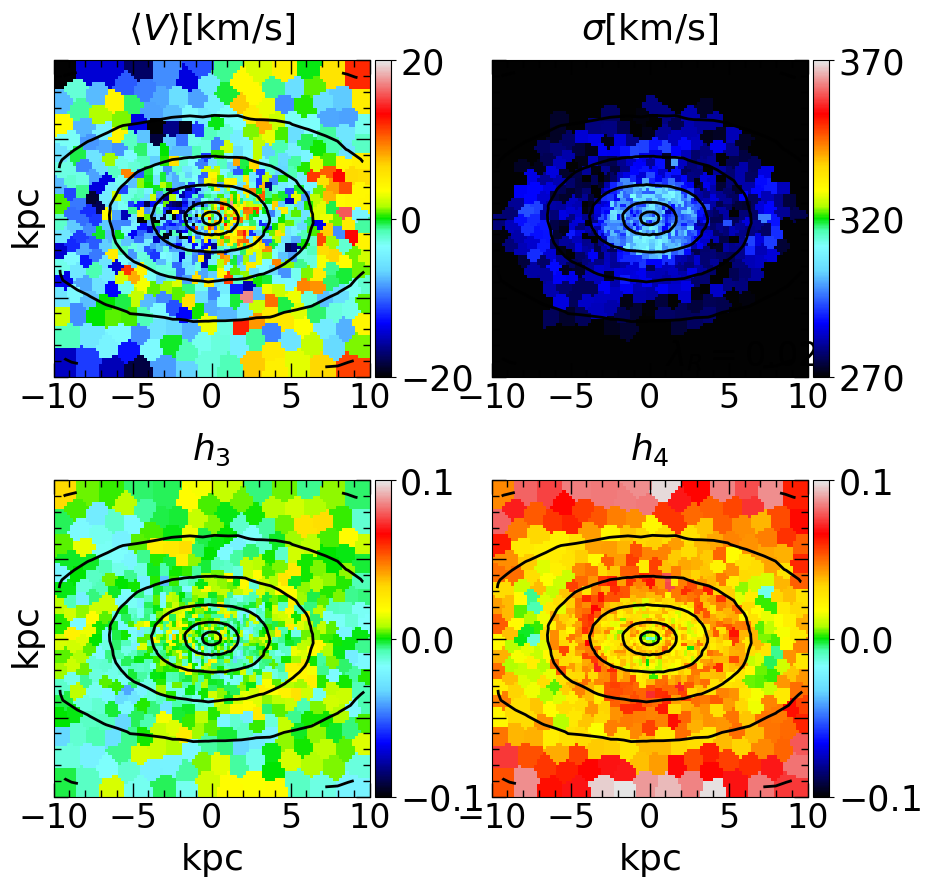
\includegraphics[width=\textwidth]{BH_1.png}
		\caption{Snapshot-1}
	\end{subfigure}
	\begin{subfigure}[b]{0.49\textwidth}
		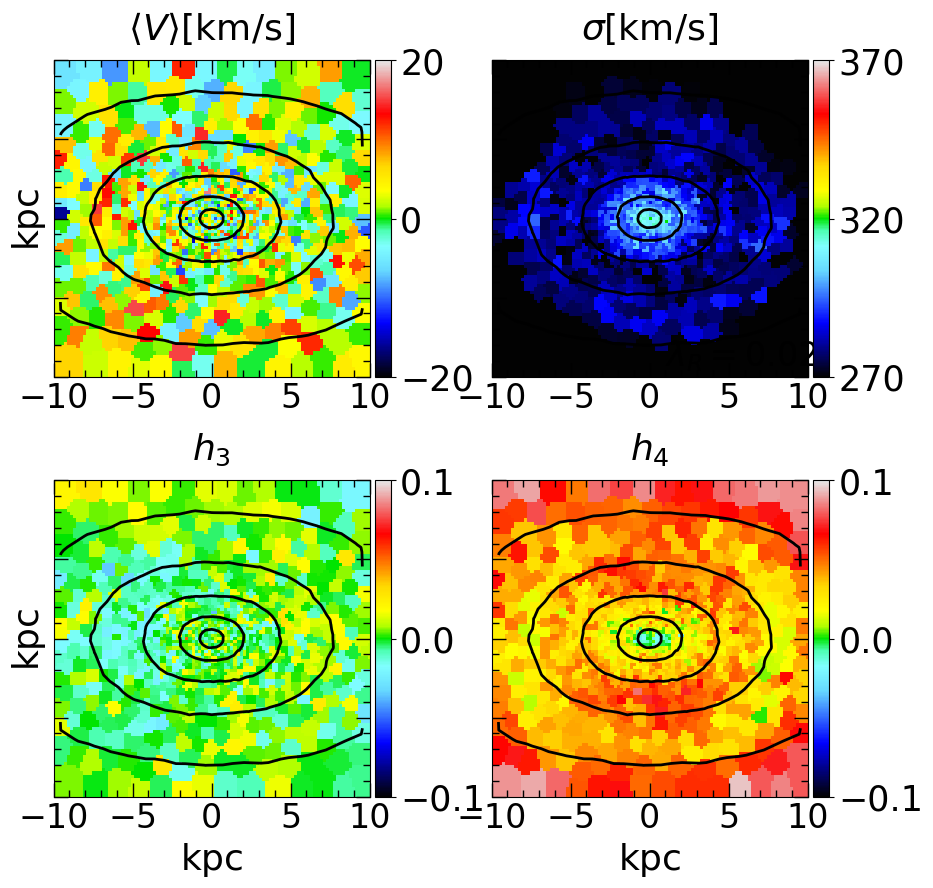
\includegraphics[width=\textwidth]{BH_2.png}
		\caption{Snapshot-2}
	\end{subfigure}
	\begin{subfigure}[b]{0.49\textwidth}
		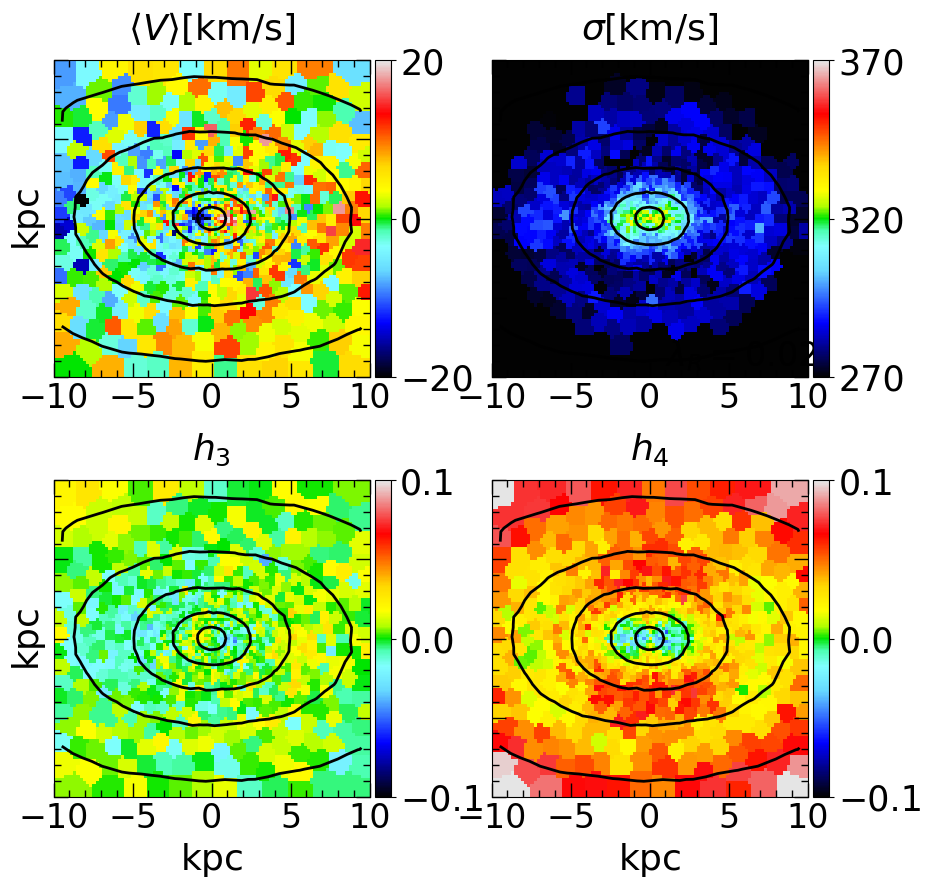
\includegraphics[width=\textwidth]{BH_3.png}
		\caption{Snapshot-3}
	\end{subfigure}
	\caption{IFU-maps of average LOS-velocities, velocity dispersion, $h_3$ parameters and $h_4$ parameters from four simulated merger remnants: Snapshot-0, Snapshot-1, Snapshot-2 and Snapshot-3.}
	\label{figure:all_voronoi_1}
\end{figure}

\begin{figure}
	\centering
	\begin{subfigure}[b]{0.49\textwidth}
		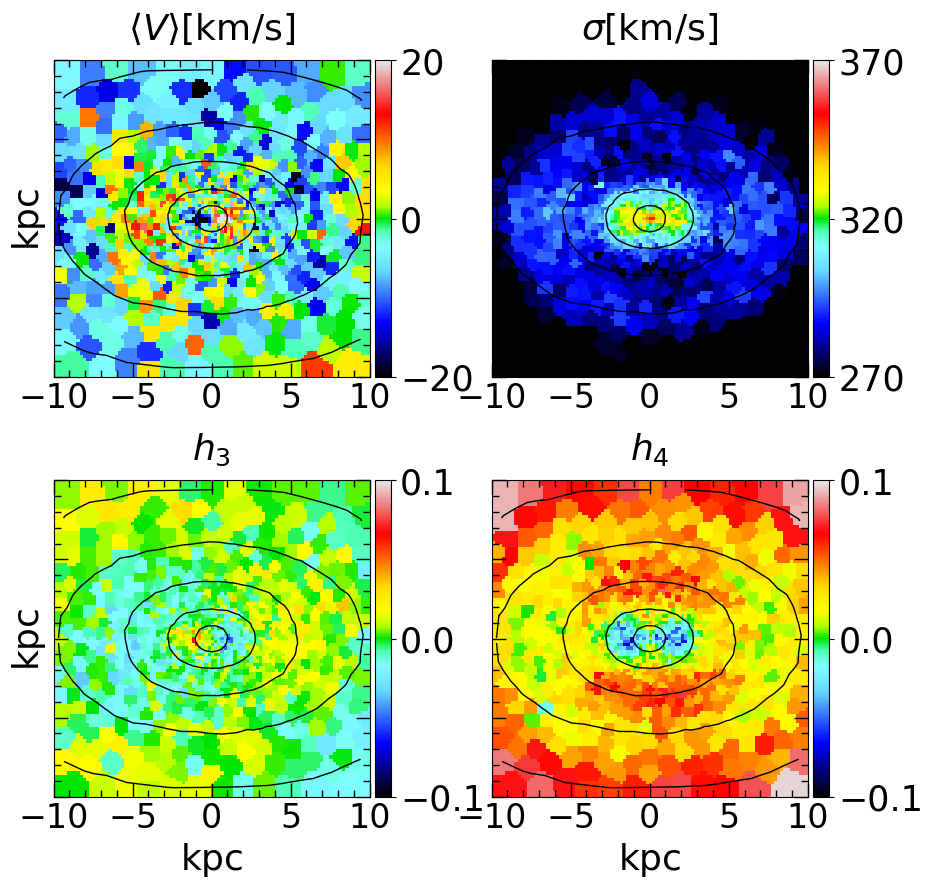
\includegraphics[width=\textwidth]{BH_4.png}
		\caption{Snapshot-4}
	\end{subfigure}
	\begin{subfigure}[b]{0.49\textwidth}
		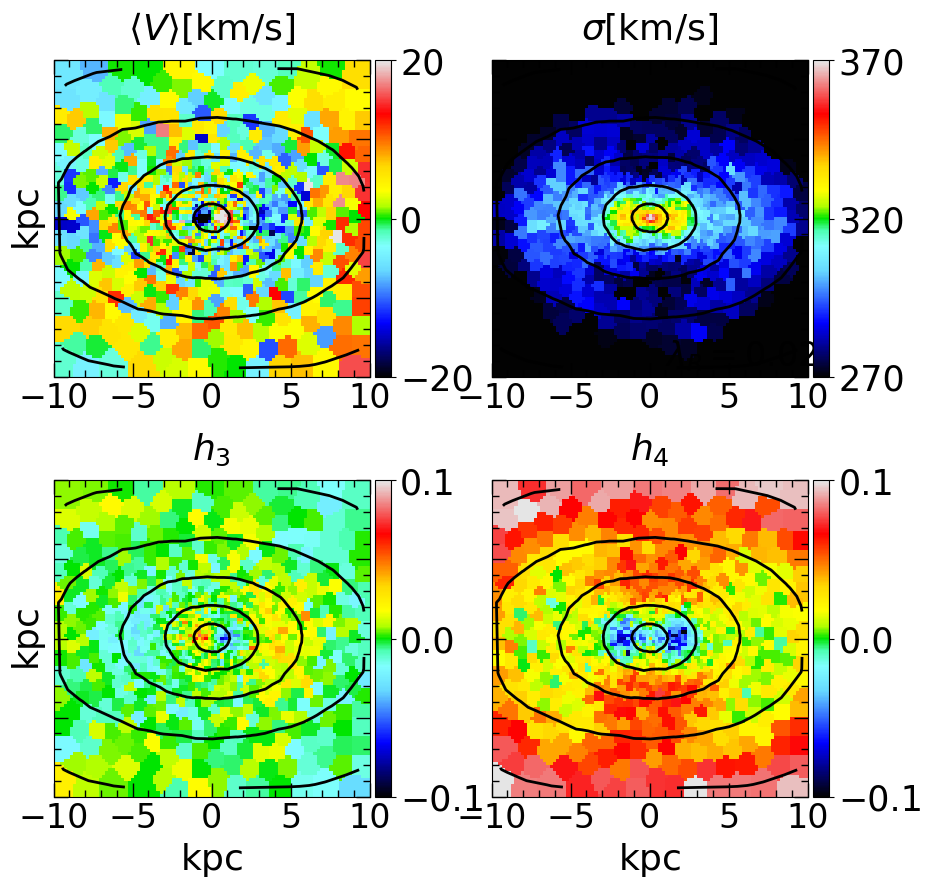
\includegraphics[width=\textwidth]{BH_5.png}
		\caption{Snapshot-5}
	\end{subfigure}
	\begin{subfigure}[b]{0.49\textwidth}
		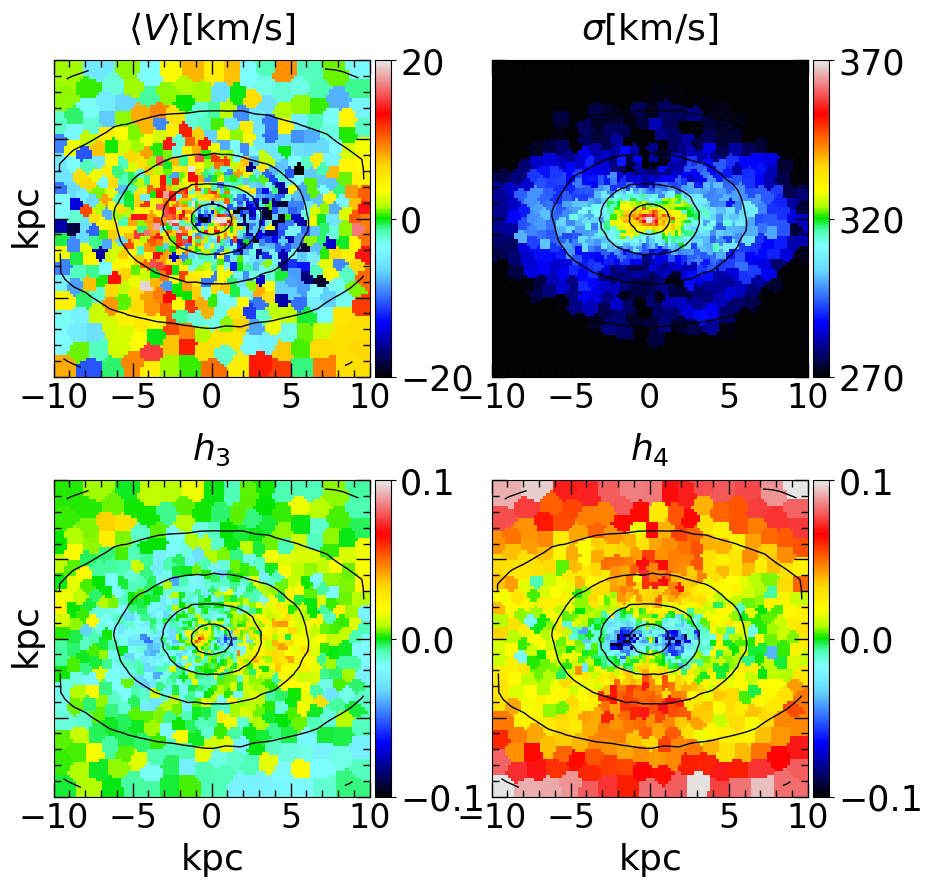
\includegraphics[width=\textwidth]{BH_6.png}
		\caption{Snapshot-6}
	\end{subfigure}
	\caption{IFU-maps of average LOS-velocities, velocity dispersion, $h_3$ parameters and $h_4$ parameters from three simulated merger remnants: Snapshot-4, Snapshot-5 and Snapshot-6.}
	\label{figure:all_voronoi_2}
\end{figure}

% STEP 5:
% Uncomment the following lines and set your .bib file and desired bibliography style
% to make a bibliography with BibTeX.
% Alternatively you can use the thebibliography environment if you want to add all
% references by hand.


% Define journal names
\newcommand{\apj}{The Astrophysical Journal}
\newcommand{\mnras}{Monthly Notices of the Royal Astronomical Society}
\newcommand{\apjs}{The Astrophysical Journal Supplement}
\newcommand{\nat}{Nature}
\newcommand{\aj}{The Astronomical Journal}
\newcommand{\na}{New Astronomy}
\newcommand{\araa}{Annual Review of Astronomy and Astrophysics}

\clearpage
\addcontentsline{toc}{chapter}{Bibliography} % This lines adds the bibliography to the ToC
\bibliographystyle{plainnat}
\bibliography{bibliography.bib}


\end{document}

